\clearpage
\chapter{Results}\label{chap:results}

\section{Overview}

Over 1 billion games were simulated in the process of evaluating the chromosomes
in this experiment. One thousand generations were evolved for every combination
of chromosome type (RGA, SGA, and TGA), population size (32, 128, 512, and
1024), number of games played by each chromosome per generation (7, 25, 50,
100), and fitness evaluator (FINISH\_ORDER (FO), NET\_WORTH (NetW),
NUM\_MONOPOLIES (NM), NUM\_PROPERTIES (NP), and NUM\_WINS (NW). In this chapter,
those four features are used to identify the different populations: for example,
RGA-512-50-NP refers to the RGA chromosome population of size 512, where each
player played 50 games per generation and the fitness evaluator was
NUM\_PROPERTIES. Results of the evolutionary process are presented in
Section~\ref{6_evoresults}.

The sixth fitness evaluator, TOURNAMENT (TO) was also tested. For the tournament
fitness evaluator the number of games was determined by the population size and
the results of each tournament, and so was not independent. When the fitness
evaluator was TO, each generation was an entire modified single elimination
tournament as described in Section~\ref{5_fitnesseval}. For TO, 1000 generations
were evolved for every combination of population size and chromosome type.

Results of the evolution of the RGA chromosome are presented first. An analysis
of the fitness distributions and descriptive statistics for various RGA
populations shows that the chromosomes are evolving.

Results for the SGA chromosomes are presented next, even though players with
this chromosome tended to evolve poorly. This is most likely due to the fact
that the data structure used for the SGA chromosomes is not well suited to the
problem domain.

Finally, results for the TGA chromosomes are briefly discussed, but these
players were essentially identical to the RGA chromosomes and so do not provide
any additional insight.

After the evolutionary process was complete, the best players from each
generation were competed in various combinations to validate the results. The
validation process is listed below. The validation of the evolved players
focuses exclusively on results obtained from the RGA chromosomes because the
SGA and TGA players do not provide any useful information.

\begin{enumerate}
  \item {Intra-population validation}
  \begin{enumerate}
    \item {For each RGA population select the best player from generation 250,
    500, 750, and 999}
    \item {Compete the 4 players in 1000 games}
    \item {Record the fitness scores for FINISH\_ORDER and NUM\_WINS}
    \item {Repeat 50 times without evolution}
    \item {Use Student's t-test to compare average fitness}
  \end{enumerate}
  \item {Inter-population validation}
  \begin{enumerate}
    \item {From generation 999 of a set of populations differing only by
    original fitness evaluator, select the best player under each fitness
    evaluator (6 players are selected)}
    \item {Create partial permutations of the 6 players taken 4 at a time}
    \item {Compete each set of 4 players in 50 games}
    \item {Record the fitness scores for FINISH\_ORDER}
    \item {Repeat 30 times without evolution}
    \item {Use Student's t-test to compare average fitness}
  \end {enumerate}
  \item {Real-world validation 1}
  \begin{enumerate}
    \item {Pick the 3 best players from the RGA-1024-100-FO population}
    \item {Select parameters for the trading algorithm}
    \item {Compete these players against human players}   
    \item {Record the finish order}
    \item {Compare average finish order and number of wins among all players}
  \end{enumerate}
  \item {Real-world validation 2}
  \begin{enumerate}
    \item {Select the top 4 players from generations 250, 500, 750, and 999 of 
    the RGA-1024-100-FO population}
    \item {Compete the players randomly against human players}
    \item {Record the finish order}
    \item {Compare average finish order and number of wins among all players}
  \end {enumerate}
  \item {Real-world validation 3}
  \begin{enumerate}
    \item {Select the top 4 players from generation 999 of the RGA-1024-100-FO
    population}
    \item {Compete the players randomly against human players}
    \item {Record the finish order}
    \item {Compare average finish order and number of wins among all players}
  \end {enumerate}
\end{enumerate}

First, an intra-population validation was performed where the best players from
different generations within a population were competed against each other.
For example, using the RGA-1024-100-NetW population (a population of RGA players
of size 1024, evolved using 100 games per generation, with the NET\_WORTH
fitness evaluator) select the best player from generations 250, 500, 750, and
999. Compete those 4 players in a set of 1000 games and record the cumulative
fitness using FINISH\_ORDER and NUM\_WINS\footnote{Regardless of the original
fitness evaluator used in evolution, the validation experiments use
FINISH\_ORDER and NUM\_WINS to compare players.}. Repeat this process 50 times
without further evolution of the players. The players' performance over the 50
trials is then analyzed to determine if players in later generations were better
than players in earlier generations. Results from this validation are discussed
in Section~\ref{6_intraPopValidation}.

Second, players were also validated with an inter-population validation. That
is, the best players from different populations were competed against each other
in various combinations. For example, given the various RGA-1024-100-*
populations, select the best player from each fitness evaluator and from
generation 999. This will select 6 players. These 6 players are then divided
into sets of 4 using partial permutations. Each set of 4 players then play 50
games; the cumulative fitness is recorded using FINISH\_ORDER. Repeat this
process 30 times without further evolution of the players\footnote{The results
of the first validation were extremely strong, which implied that 50 trials and
1000 games per trial was excessive; thus the validation parameters were relaxed
for the second validation.}. The players' performance over the 30 trials was
analyzed to determine if different fitness evaluators were better than others.
The results of this analysis can be found in Section~\ref{6_interPopValidation}.

In Section~\ref{6_humanValidation}, results from games where RGA players played
against human players are presented. Based on the previous intra- and
inter-population validations performed, the 3 best players from the
RGA-1024-100-FO population were selected. These players competed against human
players in two trials. The results are documented in Section~\ref{6_humanVRGA1}.
In general, even though the RGA players competed well against other RGA
players, they did relatively poorly against human players. This was probably
due to the property trading algorithm that was implemented for this competition.

After the first set of validation competitions, an effort was made to improve
the performance of the AI players. Four players each were picked from
generations 250, 500, 750, and 999 of the RGA-1024-100-FO population. These
players were competed against human players. There was a little improvement in
the performance of the AI players. The results of these games are documented in
Section~\ref{6_humanVRGA2}.

The property trading algorithm was adjusted again and a third competition was
performed, again using only the best players from the last generation of a
population. With the adjusted trading algorithm, the performance of the AI
players improved over the second validation. One computer player was able to
outplay the human players. The results of the third competition are documented
in the Section~\ref{6_humanVRGA3}.

\section{Results of the Evolutionary Process}\label{6_evoresults}

In this section the results of the evolutionary process are presented. Looking at
the fitness distributions and the chromosomes at the completion of evolution
shows that the players did evolve and did learn to buy some properties with greater
probability than others.

\subsection{Results for Initial RGA Generations}

In a competitive fitness evolutionary process, the individuals in the population
should be randomly spread in their fitness. When competing against each other,
some individuals will win, some will lose, and the average individual will win
about half of the competitions. The distribution of fitness scores should follow
a distribution similar to the binomial distribution (See
Figure~\ref{figure-binomial}).

When the initial populations of players was run through a single generation, the
actual results matched the expected results quite closely.

Figure~\ref{figure-RGA-G000-N100-FO-initial_fitness} shows the fitness
distribution for the first generation of the RGA-1024-100-FO population. The
figure shows a binomial shaped distribution which is centered around the
population average of 150\footnote{Because the FINISH\_ORDER evaluator assigns
1, 2, and 3 points to the players in a game, for a total of 6 points per game,
the average fitness for any single game is \(6/4\) or 1.5. So for \(n\) games
the average fitness is \(n \cdot 1.5\). For a population that plays 100 games
per generation, the fitness distribution will be centered on the average score
of 150.}.

\begin{figure}
\centering
%%----start of first figure----
\begin{minipage}[t]{0.47\linewidth}
\centering
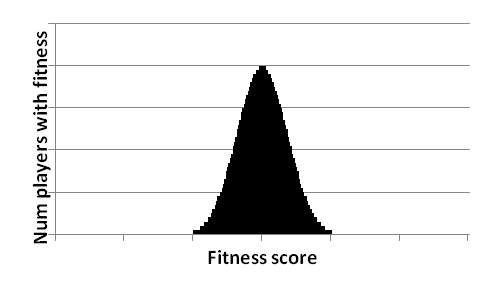
\includegraphics[width=1.0\linewidth]{Figures/binomial.png}
\caption[Binomial Distribution]{An example of the expected fitness distribution
for the first generation of a population that uses a competitive fitness
function such as FINSIH\_ORDER or NUM\_WINS. A peak is expected around the
average population fitness. The distribution is similar to a binomial
distribution.}
\label{figure-binomial}
\end{minipage}%
\hspace{0.06\linewidth}%
%%----start of second figure----
\begin{minipage}[t]{0.47\linewidth}
\centering
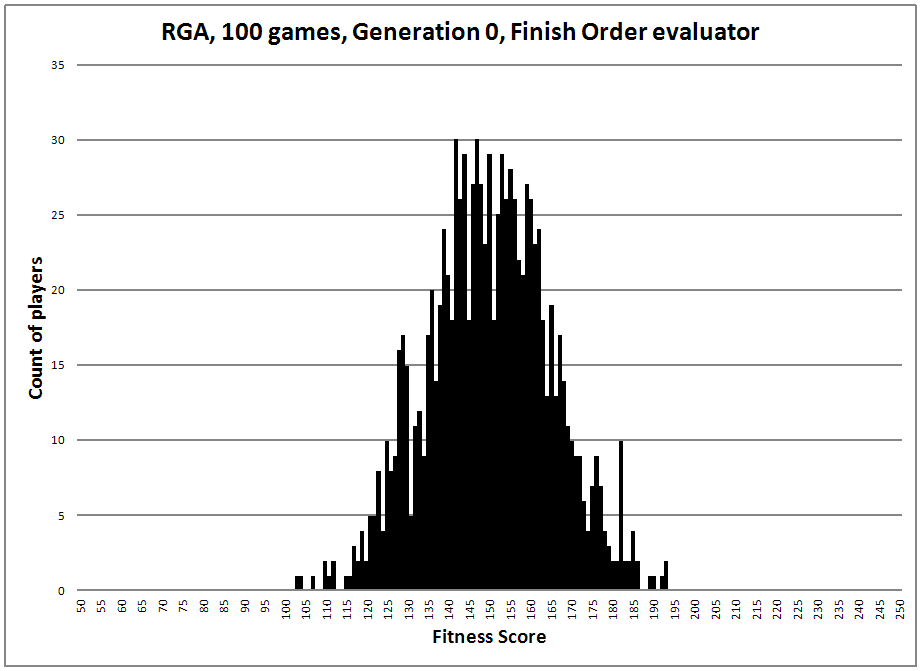
\includegraphics[width=1.0\linewidth]{Figures/RGA_1024_G000_N100_FO.png}
\caption[RGA Finish Order Fitness Distribution, Initial Generation]{RGA
chromosome, size 1024, 100 games per generation, finish order
fitness evaluator, generation 0.}
\label{figure-RGA-G000-N100-FO-initial_fitness}
\end{minipage}
\end{figure}

An example of the fitness distribution for the NUM\_WINS fitness evaluator is
shown in Figure~\ref{figure-RGA-G000-N100-NW-initial_fitness}. The average
fitness for a single game is \(3/4\) or 0.75; for \(n\) games the average
fitness is \(n \cdot 1.5\). The figure shows a binomial shaped distribution
which is centered around the population average of 75.

\begin{figure}
\centering
%%----start of first figure----
\begin{minipage}[t]{0.47\linewidth}
\centering
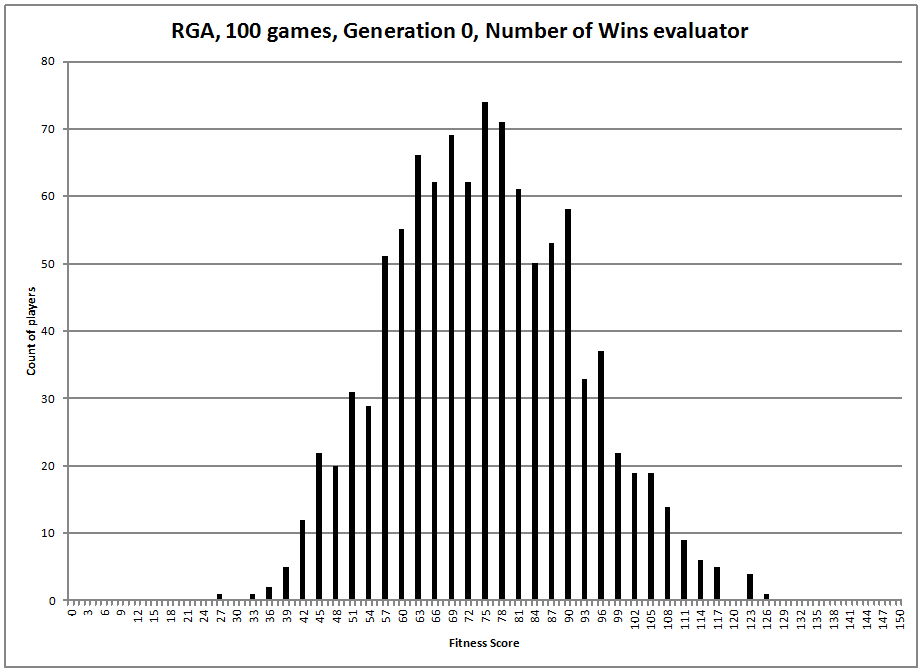
\includegraphics[width=1.0\linewidth]{Figures/RGA_1024_G000_N100_NW.png}
\caption[RGA Num Wins Fitness Distribution, Initial Generation]{RGA chromosome,
size 1024, 100 games per generation, number of wins fitness evaluator,
generation 0.}
\label{figure-RGA-G000-N100-NW-initial_fitness}
\end{minipage}%
\hspace{0.06\linewidth}%
%%----start of second figure----
\begin{minipage}[t]{0.47\linewidth}
\centering
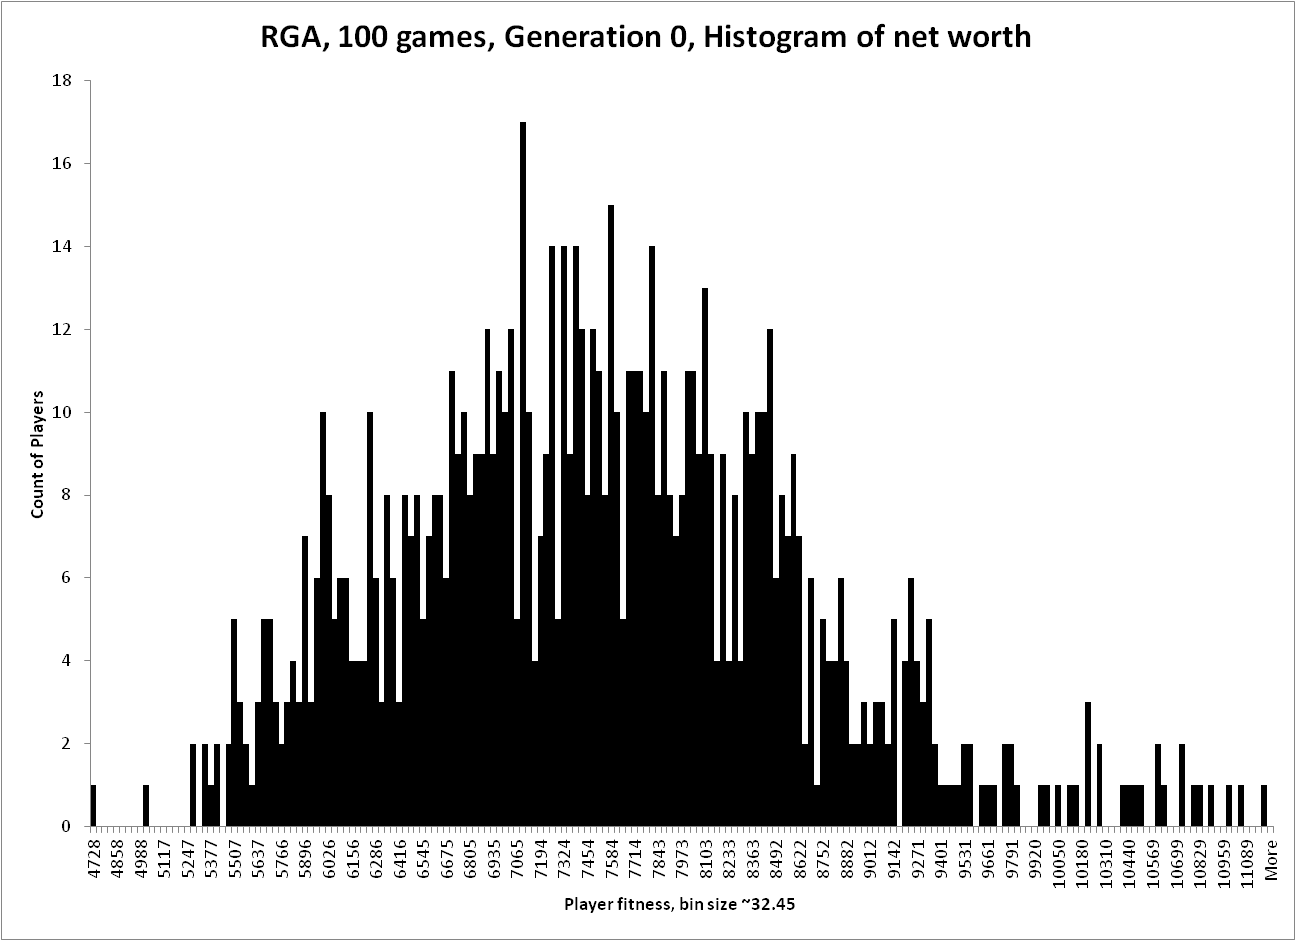
\includegraphics[width=1.0\linewidth]{Figures/RGA_1024_G000_N100_NetW.png}
\caption[Historgram of RGA Net Worth Fitness Distribution, Initial
Generation]{RGA chromosome, size 1024, 100 games per generation, net worth
fitness evaluator, generation 0.}
\label{figure-RGA-G000-N100-NetW-initial_fitness}
\end{minipage}
\\[\intextsep]

\begin{minipage}[t]{0.47\linewidth}
\centering
%%----start of third figure----
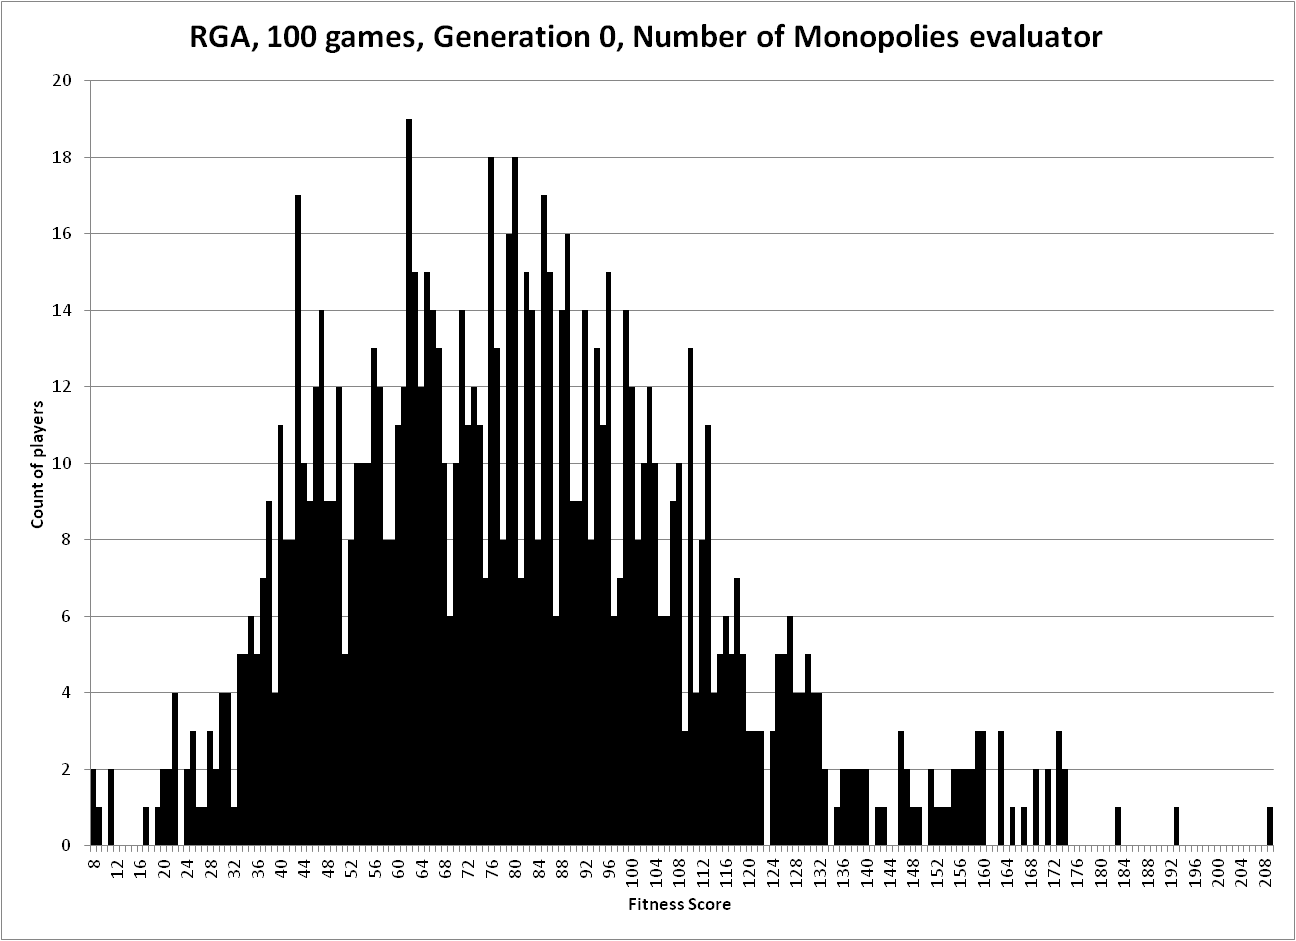
\includegraphics[width=1.0\linewidth]{Figures/RGA_1024_G000_N100_NM.png}
\caption[RGA Num Monopolies Fitness Distribution, Initial Generation]{RGA
chromosome, size 1024, 100 games per generation, number of monopolies
evaluator, generation 0.}
\label{figure-RGA-G000-N100-NM-initial_fitness}
\end{minipage}%
\hspace{0.06\linewidth}%
%%----start of fourth figure----
\begin{minipage}[t]{0.47\linewidth}
\centering
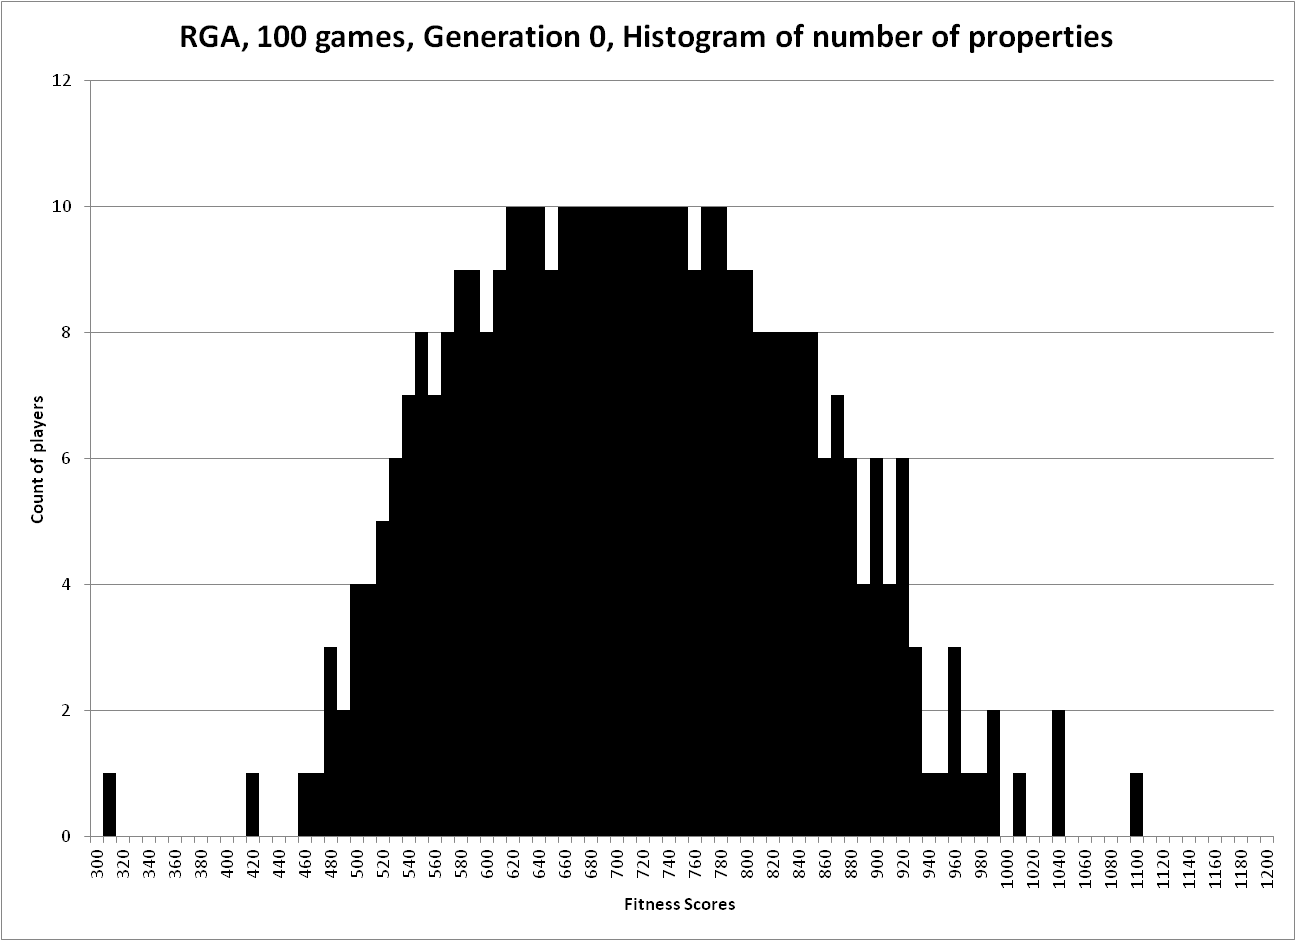
\includegraphics[width=1.0\linewidth]{Figures/RGA_1024_G000_N100_NP.png}
\caption[RGA Num Properties Fitness Distribution, Initial Generation]{RGA
chromosome, size 1024, 100 games per generation, number of properties fitness
evaluator, generation 0.}
\label{figure-RGA-G000-N100-NP-initial_fitness}

\end{minipage}
\end{figure}

Example fitness distributions for the other fitness evaluators are shown in
Figure~\ref{figure-RGA-G000-N100-NetW-initial_fitness},
Figure~\ref{figure-RGA-G000-N100-NM-initial_fitness}, and
Figure~\ref{figure-RGA-G000-N100-NP-initial_fitness}. The distribution for
TOURNAMENT is not shown because it provides no useful information. For
TOURNAMENT, half the population has a score of 0, half of the remainder has a
score of 1, etc., until the final two players have a score of \(log_{2} n-1\).
The TOURNAMENT population will be discussed more in the validation section.

All of the other populations, regardless of population size, fitness evaluator,
or number of games per generation, show similar results for the initial
generation. These fitness distributions are not surprising. Four of the fitness
evaluators are competitive fitness functions (NUM\_MONOPOLIES and
NUM\_PROPERTIES are not directly competitive, since the player with the most
monopolies or properties is not necessarily the winner of the game). The fact
that the results match previous research into competitive fitness functions
shows that the evolutionary approach that was taken appears to be correct.

\subsection{Results for Subsequent RGA Generations}

In a population that co-evolves under a competitive fitness function, the
average and best scores in the population will not increase. As poor players are
removed from the population, the remaining players will tend to be nearer each
other in ``ability.'' Thus, the distribution of fitness scores will become much
tighter around the average score, and no single player will be able to dominate
the other players.

This is seen in all the RGA populations. As the populations evolved, the
variance in fitness scores in later generations tended to decrease. A
representative example of this can be seen in generation 100 of the
RGA-1024-100-FO population. Figure~\ref{figure-100th_gen_fitness} shows the
actual fitness distribution for this population. The mean remained the same, but
the variance has appeared to decrease. Whereas the fitness scores in generation
0 ranged from 103 to 193, in generation 100 they ranged from 115 to 186. The
distribution around the mean tightened relatively quickly (it can clearly be
seen in generation 100). 

\begin{figure}[htp]
\centerline{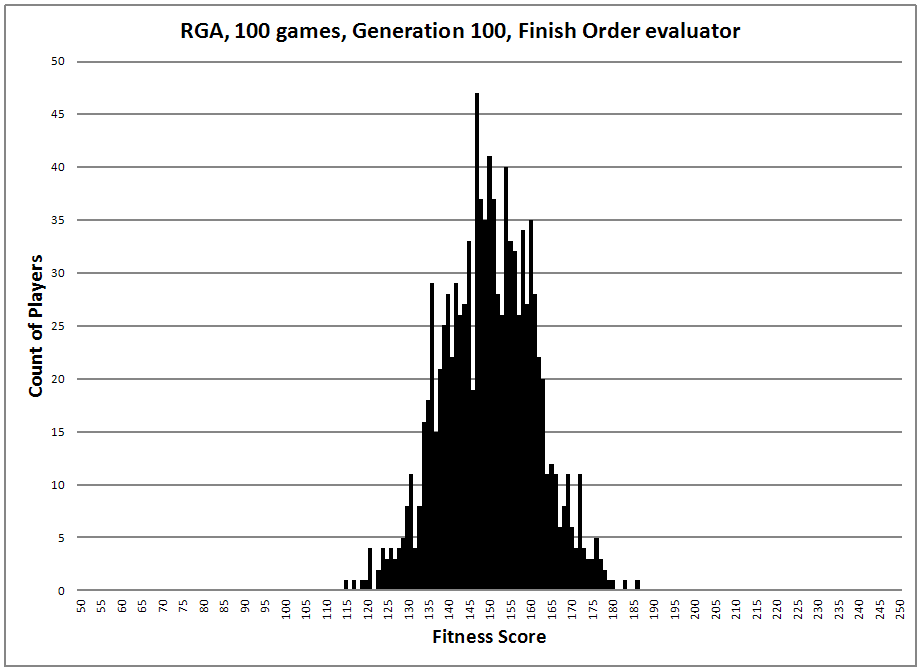
\includegraphics[width=0.75\columnwidth]{Figures/RGA_1024_G100_N100_FO.png}}
\caption[RGA Fitness Distribution, 100th Generation]{RGA chromosome, generation
100, 100 games per generation, finish order fitness evaluator.}
\label{figure-100th_gen_fitness}
\end{figure}

This behavior remained fairly constant over the remaining generations.
Additional plots of the distribution of fitness scores can be seen in
Figure~\ref{figure-RGA-250th_gen_fitness},
Figure~\ref{figure-RGA-500th_gen_fitness},
Figure~\ref{figure-RGA-750th_gen_fitness}, and
Figure~\ref{figure-RGA-999th_gen_fitness}. Each of these figures shows the
RGA-1024-100-FO population at various points in the evolution process.

\begin{figure}
\centering
%%----start of first figure----
\begin{minipage}[t]{0.47\linewidth}
\centering
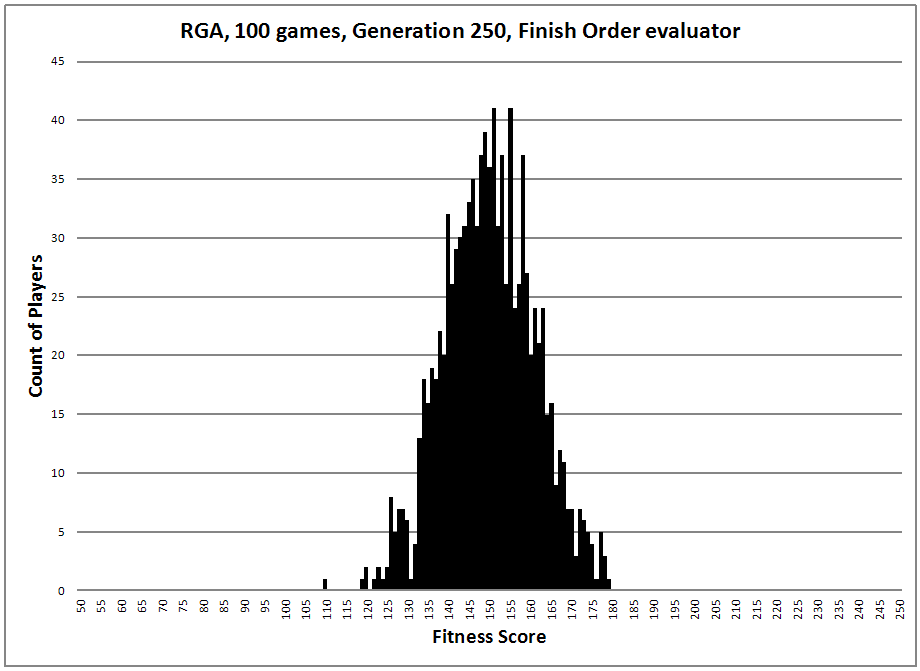
\includegraphics[width=1.0\linewidth]{Figures/RGA_1024_G250_N100_FO.png}
\caption[RGA Fitness Distribution, 250th Generation]{RGA chromosome, size 1024,
100 games per generation, finish order fitness evaluator, generation
250.}
\label{figure-RGA-250th_gen_fitness}
\end{minipage}%
\hspace{0.06\linewidth}%
%%----start of second figure----
\begin{minipage}[t]{0.47\linewidth}
\centering
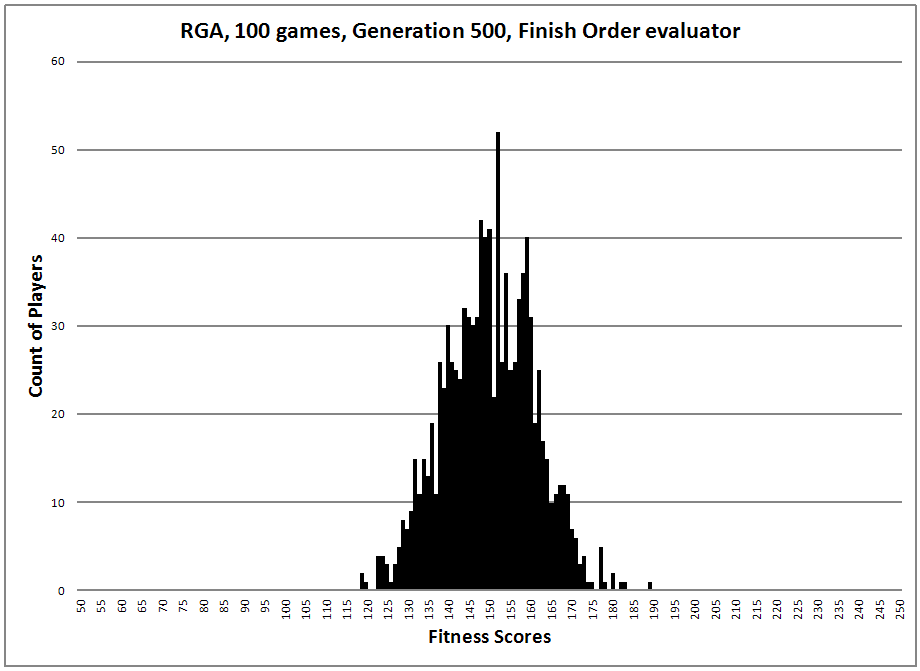
\includegraphics[width=1.0\linewidth]{Figures/RGA_1024_G500_N100_FO.png}
\caption[RGA Fitness Distribution, 500th Generation]{RGA chromosome, size 1024,
100 games per generation, finish order fitness evaluator, generation
500.}
\label{figure-RGA-500th_gen_fitness}
\end{minipage}

\begin{minipage}[t]{0.47\linewidth}
\centering
%%----start of third figure----
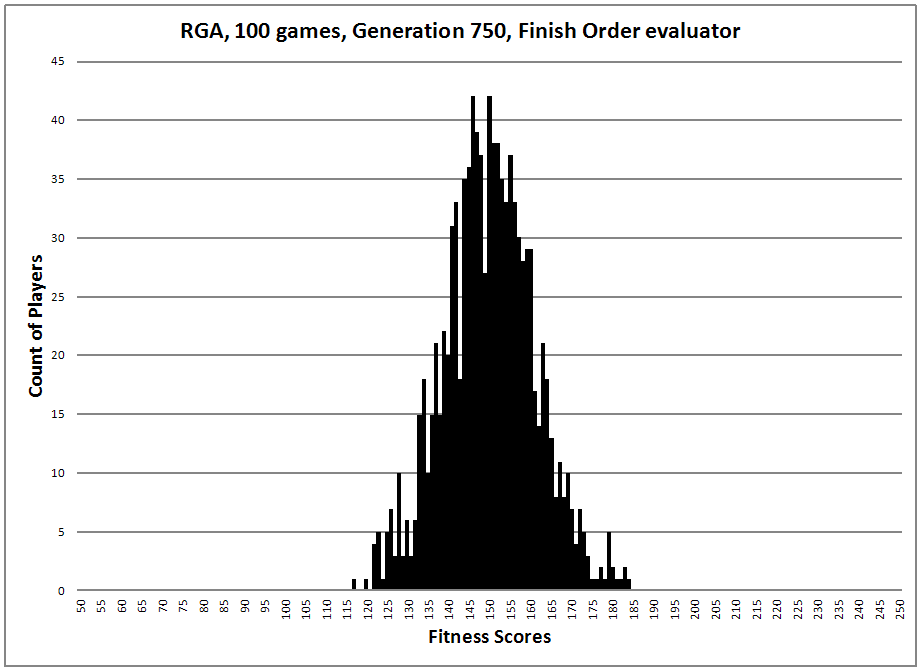
\includegraphics[width=1.0\linewidth]{Figures/RGA_1024_G750_N100_FO.png}
\caption[RGA Fitness Distribution, 750th Generation]{RGA chromosome, size 1024,
100 games per generation, finish order fitness evaluator, generation
750.}
\label{figure-RGA-750th_gen_fitness}
\end{minipage}%
\hspace{0.06\linewidth}%
%%----start of fourth figure----
\begin{minipage}[t]{0.47\linewidth}
\centering
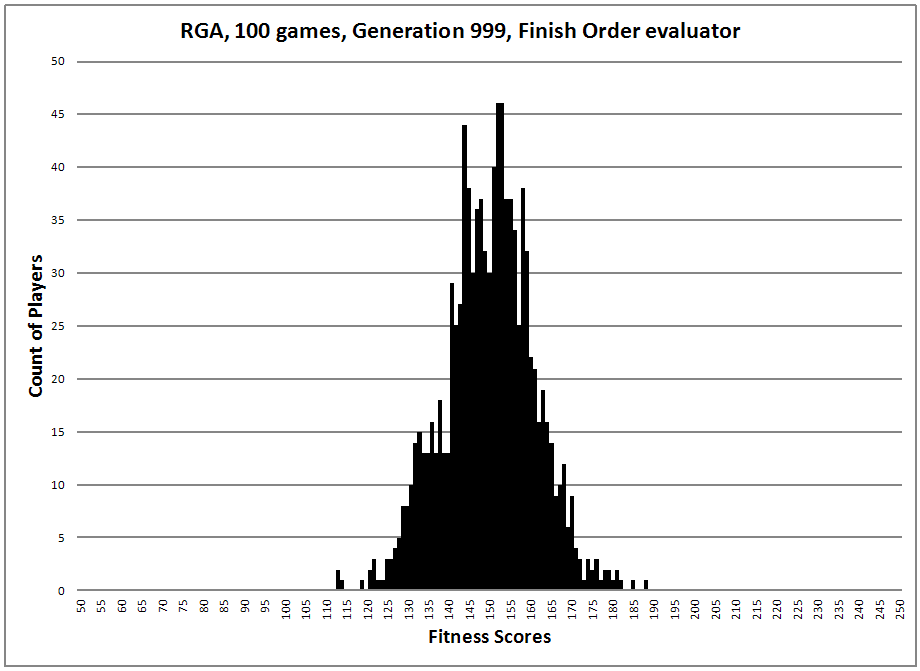
\includegraphics[width=1.0\linewidth]{Figures/RGA_1024_G999_N100_FO.png}
\caption[RGA Fitness Distribution, 999th Generation]{RGA chromosome, size 1024,
100 games per generation, finish order fitness evaluator, generation
999.}
\label{figure-RGA-999th_gen_fitness}
\end{minipage}
\end{figure}

Inspecting Figures~\ref{figure-RGA-250th_gen_fitness} through
\ref{figure-RGA-999th_gen_fitness}, it appears that at some point between the
100th generation and the 250th generation\footnote{Because of the large amount
of data generated by the simulations, data for every generation was not output
by the simulation. Instead fitness data was output and saved for the initial
population, the 100th generation, and every 250th generation. Thus, the point at
which the population average fitness reaches the plateau cannot be calculated.}
that the population average fitness reaches a plateau. This is also demonstrated
by looking at some of the descriptive statistics for each generation. These are
shown in Table~\ref{table-stats-for-s1024-n100-fo} for the RGA-1024-100-FO
population.

\begin{table}[ht]
\begin{center}
\caption[RGA-1024-100-FO statistics]{Descriptive statistics for RGA-1024-100-FO}
\begin{tabular}{ | r || r | r | r | r | r |}
\hline
Generation & Min & Max & Average & Variance & Std Dev \\ \hline \hline
0   & 103 & 193 & 150 & 227.43 & 15.08 \\ \hline
100 & 115 & 186 & 150 & 126.81 & 11.26 \\ \hline
250 & 110 & 179 & 150 & 122.02 & 11.05 \\ \hline
500 & 119 & 189 & 150 & 120.44 & 10.97 \\ \hline
750 & 117 & 184 & 150 & 124.63 & 11.16 \\ \hline
999 & 113 & 188 & 150 & 121.10 & 11.00 \\ \hline
\end{tabular}
\label{table-stats-for-s1024-n100-fo}
\end{center}
\end{table}

In the initial generation, the standard deviation is 15.08, it drops to 11.26 by
the 100th generation, and then in the remaining generations (250, 500, 750, and
999) the standard deviation appears to fluctuate around 11.05. No test was
made to determine whether this difference in variance between
generations is statistically significant\footnote{To test the hypothesis that the standard
deviations are not equal between generations would require running (in this
example) a population of size 1024 through at least 250 generations, and then
repeating that 250 generation trial enough times to get a statistically
significant sample. Based on the work performed for this research, doing this
for all of the populations would have taken several weeks of processing
time. It was decided that a better use of resources would be to do a comparative
test between players of different generations and populations.}.

Additional population statistics are in
Table~\ref{table-stats-for-s1024-n100-netw} for the RGA-1024-100-NetW
population, Table~\ref{table-stats-for-s1024-n100-nm} for the RGA-1024-100-NM
population, Table~\ref{table-stats-for-s1024-n100-np} for the RGA-1024-100-NP
population, and Table~\ref{table-stats-for-s1024-n100-nw} for the
RGA-1024-100-NW population.

\begin{table}[ht]
\begin{center}
\caption[RGA-1024-100-NetW statistics]{Descriptive statistics for RGA-1024-100-NetW}
\begin{tabular}{ | r || r | r | r | r | r |}
\hline
Generation & Min & Max & Average & Variance & Std Dev \\ \hline \hline
0   & 4728 & 11186 & 7499.99 & 1137919.23 & 1066.73 \\ \hline
250 & 4285 & 10374 & 7499.80 &  649447.67 &  805.88 \\ \hline
500 & 5235 & 10242 & 7500.00 &  665909.43 &  816.03 \\ \hline
750 & 5080 & 10977 & 7500.05 &  723209.97 &  850.42 \\ \hline
999 & 5306 &  9831 & 7499.96 &  649001.83 &  805.61 \\ \hline
\end{tabular}
\label{table-stats-for-s1024-n100-netw}
\end{center}
\end{table}

\begin{table}[ht]
\begin{center}
\caption[RGA-1024-100-NM statistics]{Descriptive statistics for RGA-1024-100-NM}
\begin{tabular}{ | r || r | r | r | r | r |}
\hline
Generation & Min & Max & Average & Variance & Std Dev \\ \hline \hline
0   &  8 & 209 &  80.42 & 1014.77 & 31.86 \\ \hline
250 & 37 & 226 & 110.88 &  758.92 & 27.55 \\ \hline
500 & 43 & 199 & 111.20 &  707.89 & 26.61 \\ \hline
750 & 44 & 199 & 113.97 &  732.09 & 27.06 \\ \hline
999 & 17 & 217 & 116.52 &  734.49 & 27.10 \\ \hline
\end{tabular}
\label{table-stats-for-s1024-n100-nm}
\end{center}
\end{table}

\begin{table}[ht]
\begin{center}
\caption[RGA-1024-100-NP statistics]{Descriptive statistics for RGA-1024-100-NP}
\begin{tabular}{ | r || r | r | r | r | r |}
\hline
Generation & Min & Max & Average & Variance & Std Dev \\ \hline \hline
0   & 309 & 1094 & 698.18 &  10271.47 & 101.35 \\ \hline
250 & 504 &  929 & 697.75 &   5322.08 &  72.95 \\ \hline
500 & 478 &  973 & 697.72 &   6126.09 &  78.27 \\ \hline
750 & 462 &  983 & 697.81 &   5928.88 &  77.00 \\ \hline
999 & 438 & 1007 & 697.79 &   6095.32 &  78.07 \\ \hline
\end{tabular}
\label{table-stats-for-s1024-n100-np}
\end{center}
\end{table}

\begin{table}[ht]
\begin{center}
\caption[RGA-1024-100-NW statistics]{Descriptive statistics for RGA-1024-100-NW}
\begin{tabular}{ | r || r | r | r | r | r |}
\hline
Generation & Min & Max & Average & Variance & Std Dev \\ \hline \hline
0   & 27 & 126 & 75.00 & 286.43 & 16.92 \\ \hline
250 & 36 & 120 & 75.00 & 155.68 & 12.48 \\ \hline
500 & 30 & 117 & 75.00 & 168.21 & 12.97 \\ \hline
750 & 39 & 120 & 75.00 & 160.36 & 12.66 \\ \hline
999 & 30 & 114 & 75.00 & 173.74 & 13.18 \\ \hline
\end{tabular}
\label{table-stats-for-s1024-n100-nw}
\end{center}
\end{table}

In all of the tables, the average population fitness stays approximately
the same, and the variance in population fitness decreases. Even though it
appears that the variance has plateaued in these examples, players in later
generations can still be improving in fitness. In fact, 
later in this chapter statistical tests show that players in the last generation
are better (i.e., they win more games) than players in the earliest generations.

This section has focused primarily on the RGA-1024-100-* populations. In
general, a similar pattern of statistics is seen in most of the other RGA and
TGA populations that were evolved in this study. Some of the populations,
however, showed weaker, or sometimes conflicting results. A complete set of
tables with that information for the RGA populations can be found in
Appendix~\ref{appendix:rgastats}.

The populations that did not appear to improve over time were the populations
with small population size or small numbers of games per generation. One example
is shown in Table~\ref{tab:6_RGA-0032-007-FO}. In this case, the population
variance gets larger over time, which implies that this population improved
little or none from the first generation to the last. Section~\ref{6_Validation}
provides details on whether the populations did improve or not.

\begin{table}[htbp]
  \centering
  \caption[RGA-0032-007-FO Statistics]{Descriptive Statistics for RGA-0032-007-FO}
    \begin{tabular}{lrrrrrr}
    \toprule
    Population &  Generation & Min    & Max    & Average & Variance & Std Dev \\
    \midrule
    RGA-0032-007-FO & 0      & 4      & 16     & 10.50  & 8.77   & 2.96 \\
    RGA-0032-007-FO & 250    & 4      & 17     & 10.50  & 9.23   & 3.04 \\
    RGA-0032-007-FO & 500    & 5      & 16     & 10.50  & 10.13  & 3.18 \\
    RGA-0032-007-FO & 750    & 2      & 19     & 10.50  & 12.71  & 3.57 \\
    RGA-0032-007-FO & 999    & 5      & 16     & 10.50  & 10.26  & 3.20 \\
    \bottomrule
    \end{tabular}
  \label{tab:6_RGA-0032-007-FO}%
\end{table}%

\subsection{Genome Changes Over Time} \label{6_genomeChanges}

This section looks at the changes in a genome between the initial and final
generations of a population. Using the RGA-1024-100-FO population, part of
the genome for the best player from generation 0 is shown in
Figure~\ref{figure-genome0} and part of the genome for the best player from
generation 999 is shown in Figure~\ref{figure-genome999}. For easier comparison,
the chromosome values from the chart are also shown in
Table~\ref{tab:chromo_compare}.

\begin{figure}[htp]
\centerline{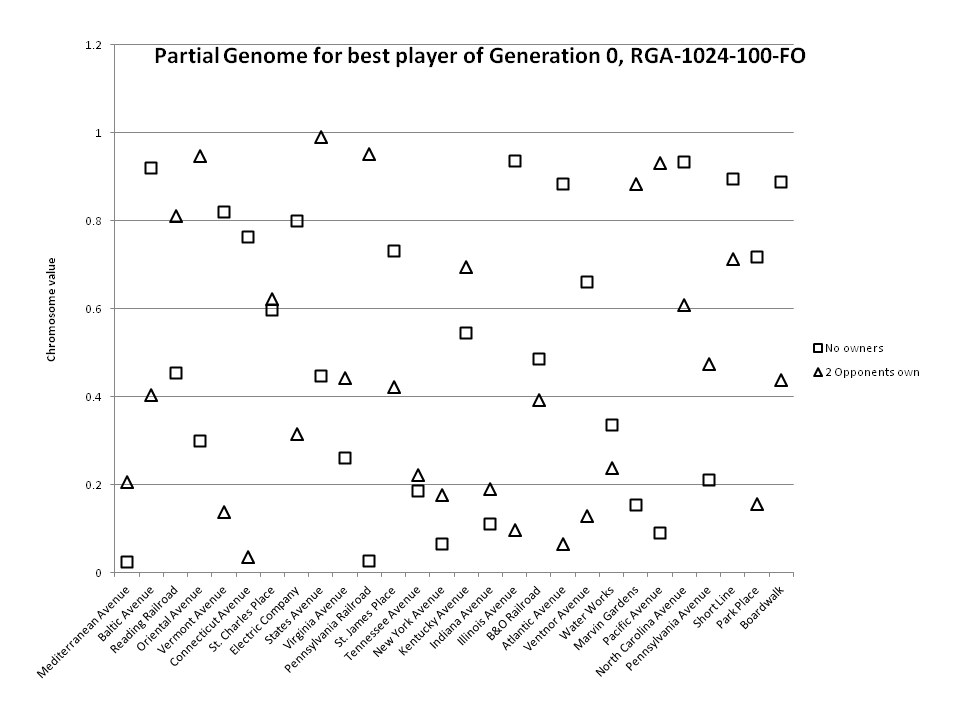
\includegraphics[width=0.85\columnwidth]{Figures/genome000.png}}
\caption[Illustration of Genome, Generation 0]{This chart shows part of the
genome of the fittest player in the first generation of the RGA-1024-100-FO
population. This chart compares the chromosome used when no player owns any
property in the group (represented by the square symbol) against the chromosome
used when two other players own a property in the group (the triangle symbol).
Note that the gene values appear to be randomly distributed in the chart.}
\label{figure-genome0}
\end{figure}

\begin{figure}[htp]
\centerline{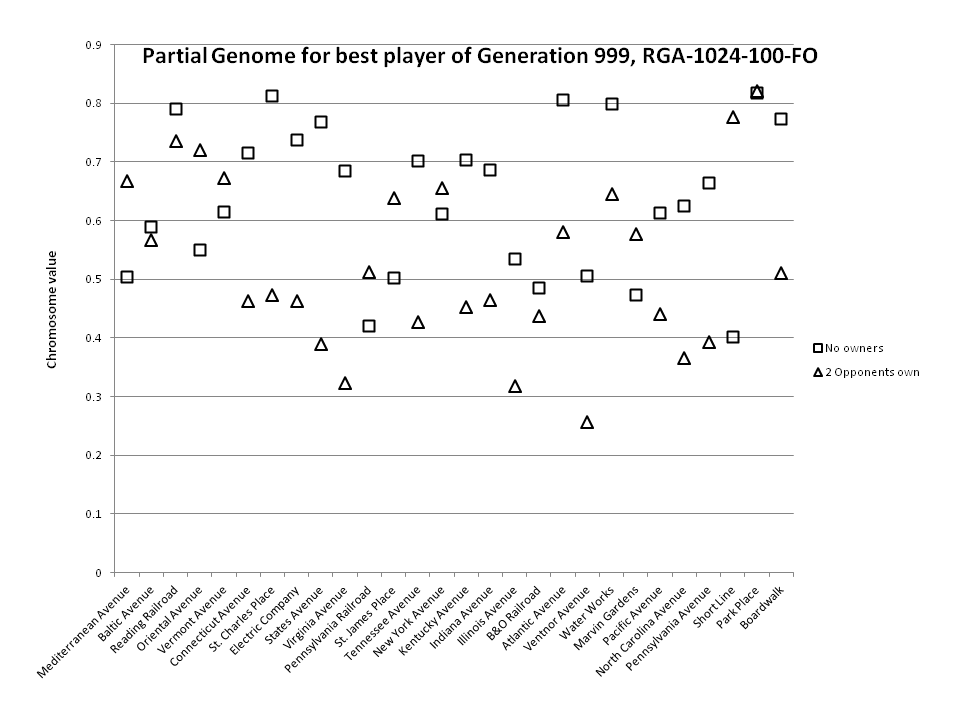
\includegraphics[width=0.85\columnwidth]{Figures/genome999.png}}
\caption[Illustration of Genome, Generation 999]{This chart shows part of the
genome of the fittest player in the last generation of the RGA-1024-100-FO
population. This chart compares the chromosome used when no player owns any
property in the group (the square symbol) against the chromosome used when two
other players own a property in the group (the triangle symbol). These two genes
show agreement with the heuristic strategy: the player is more likely to buy a
property when no one owns a property in the group, and relatively less likely to
buy a property when other players are blocking the group from being monopolized.
Note that the gene values are appear to be less random in this Figure.}
\label{figure-genome999}
\end{figure}

% Table generated by Excel2LaTeX from sheet 'genome0099 (2)'
\begin{table}[htbp]
  \centering
  \caption[Genome Comparison, Gen 0 vs Gen 999]{Comparison of Best Genomes from Generation 0 and Generation 999}
  \scalebox{0.9}{
    \begin{tabular}{lrrr|rrr}
    \toprule
           & \multicolumn{3}{c|}{Generation 0} & \multicolumn{3}{c}{Generation 999} \\
    \midrule
           & No Owner & 2 Opponents own & Diff   & No Owner & 2 Opponents own & Diff \\
    Mediterranean Avenue & 0.023  & 0.205  & -0.182 & 0.504  & 0.668  & -0.164 \\
    Baltic Avenue & 0.920  & 0.404  & 0.517  & 0.589  & 0.567  & 0.023 \\
    Reading Railroad & 0.454  & 0.810  & -0.356 & 0.790  & 0.736  & 0.054 \\
    Oriental Avenue & 0.300  & 0.947  & -0.648 & 0.550  & 0.721  & -0.171 \\
    Vermont Avenue & 0.821  & 0.138  & 0.683  & 0.614  & 0.673  & -0.059 \\
    Connecticut Avenue & 0.762  & 0.036  & 0.726  & 0.715  & 0.463  & 0.252 \\
    St. Charles Place & 0.598  & 0.622  & -0.024 & 0.812  & 0.473  & 0.339 \\
    Electric Company & 0.799  & 0.314  & 0.484  & 0.737  & 0.463  & 0.274 \\
    States Avenue & 0.448  & 0.991  & -0.543 & 0.768  & 0.389  & 0.379 \\
    Virginia Avenue & 0.260  & 0.442  & -0.182 & 0.685  & 0.323  & 0.362 \\
    Pennsylvania Railroad & 0.027  & 0.952  & -0.925 & 0.421  & 0.512  & -0.091 \\
    St. James Place & 0.730  & 0.423  & 0.308  & 0.502  & 0.639  & -0.137 \\
    Tennessee Avenue & 0.186  & 0.223  & -0.036 & 0.702  & 0.427  & 0.275 \\
    New York Avenue & 0.064  & 0.175  & -0.111 & 0.612  & 0.656  & -0.043 \\
    Kentucky Avenue & 0.544  & 0.694  & -0.150 & 0.704  & 0.452  & 0.252 \\
    Indiana Avenue & 0.110  & 0.189  & -0.080 & 0.686  & 0.465  & 0.221 \\
    Illinois Avenue & 0.936  & 0.096  & 0.840  & 0.536  & 0.319  & 0.217 \\
    B\&O Railroad & 0.487  & 0.391  & 0.095  & 0.485  & 0.437  & 0.048 \\
    Atlantic Avenue & 0.884  & 0.064  & 0.820  & 0.806  & 0.581  & 0.225 \\
    Ventnor Avenue & 0.661  & 0.128  & 0.532  & 0.506  & 0.257  & 0.250 \\
    Water Works & 0.335  & 0.237  & 0.098  & 0.800  & 0.645  & 0.154 \\
    Marvin Gardens & 0.154  & 0.883  & -0.730 & 0.472  & 0.577  & -0.104 \\
    Pacific Avenue & 0.091  & 0.931  & -0.840 & 0.614  & 0.440  & 0.173 \\
    North Carolina Avenue & 0.934  & 0.609  & 0.325  & 0.625  & 0.365  & 0.260 \\
    Pennsylvania Avenue & 0.210  & 0.474  & -0.265 & 0.663  & 0.392  & 0.271 \\
    Short Line & 0.895  & 0.713  & 0.182  & 0.402  & 0.778  & -0.376 \\
    Park Place & 0.718  & 0.155  & 0.563  & 0.818  & 0.822  & -0.004 \\
    Boardwalk & 0.887  & 0.439  & 0.448  & 0.774  & 0.511  & 0.263 \\
    \bottomrule
    \end{tabular}}
  \label{tab:chromo_compare}%
\end{table}%

For the property buying decision, the genome in Figure~\ref{figure-genome999}
matches the strategy described previously. The gene values for buying a location
are generally higher when no player owns one of the properties of a group
compared to when two other players own properties in the group. Although it is
not shown in Figure~\ref{figure-genome999}, the gene values for buying when the
player already owns a property in the group, or when one opponent owns a
property in the group, are generally higher than when two opponents own a
property in the group.

When compared to the strategy list from Section~\ref{m_gamestrategies}, there
might appear to be an inconsistency in the genome. For example, the strategy
says always buy a property if no one else owns a property in the same group.
However, the greatest gene value in the genome from generation 999 is for Park
Place at 0.82. This can easily be explained by the fact that if the player
declines a property with probability \(p_{decline} = 1-p_{buy}\), the
probability of subsequently buying the property is higher. This is because when
a player declines a property, it is then auctioned to any player including the
declining player, and the declining player uses the same chromosome to make the
bid decision independently of the buy decision. So the probability of deciding
to buy a property is
\begin{equation*}
1-(p_{decline} \cdot p_{decline})
\end{equation*}
For example, the probability of a player deciding to buy Park Place with a
gene value of 0.82 is
\begin{equation*}
1-(0.18 \cdot 0.18) \approx 0.97
\end{equation*}
The probability of actually obtaining the property is slightly lower, however,
since it is dependent on winning the auction.

\subsection{SGA Players} \label{6_SGA}

After evolving the population of RGA Players, the simulation was conducted again
using SGA Players. SGA players are those players with a binary string
chromosome.

The fitness distribution in the first generation shows the same general
similarity to the binomial distribution (Figure~\ref{figure-sga_gen0}), although
there appears to be a bit of skewness.

\begin{figure}[htp]
\centerline{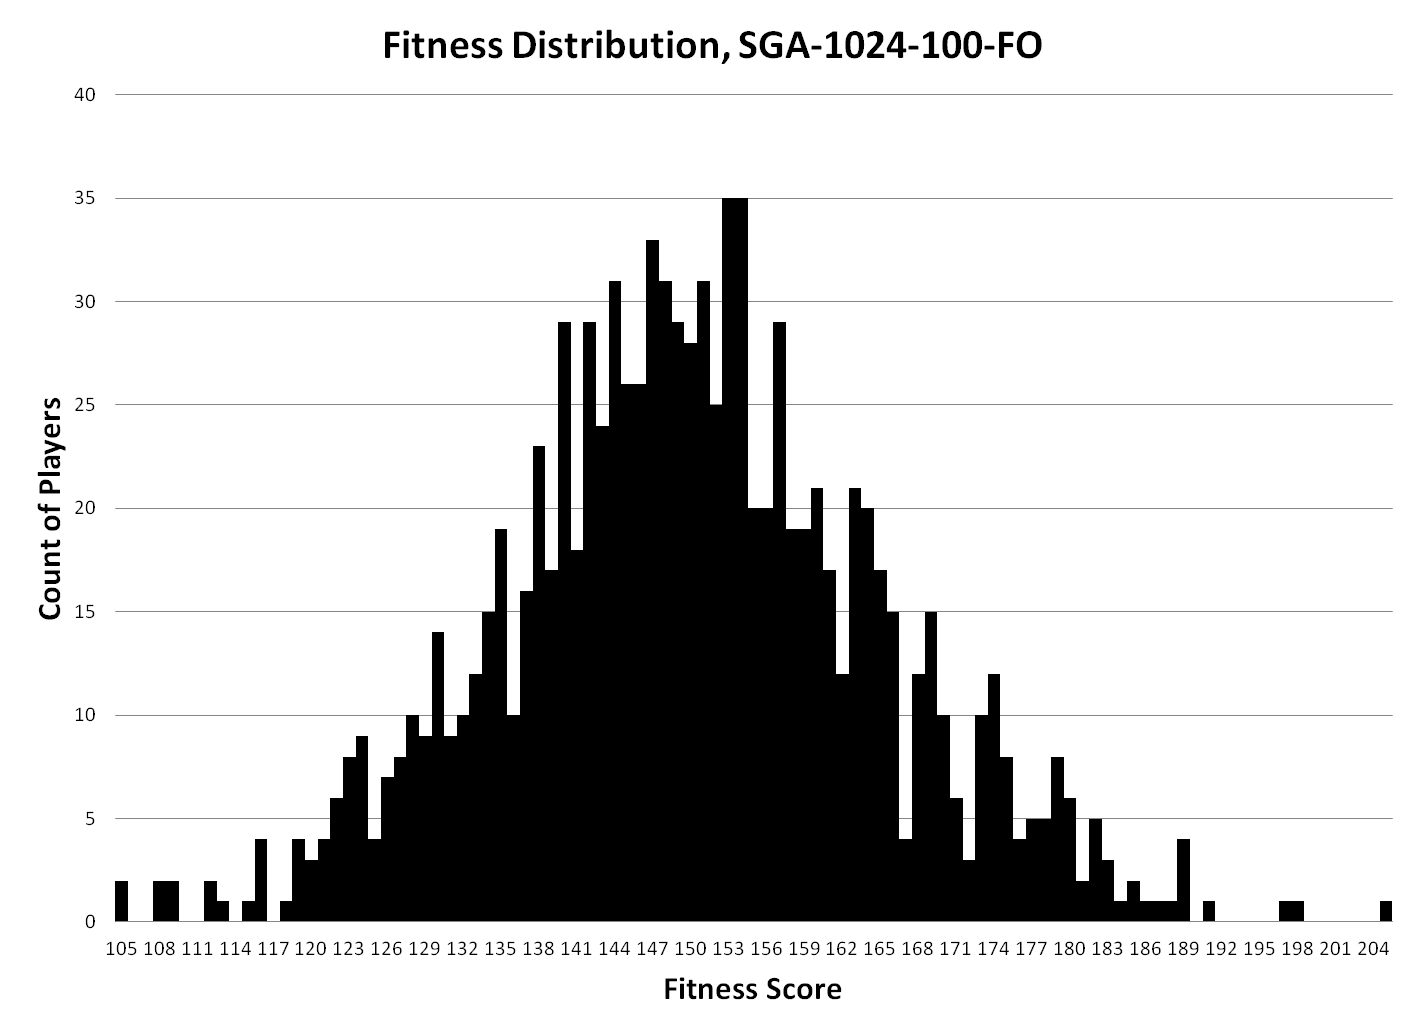
\includegraphics[width=0.75\columnwidth]{Figures/SGA_1024_100_FO_gen0.png}}
\caption[SGA-1024-100-FO Fitness Generation 0]{This figure shows the fitness
distribution for the first generation of the SGA-1024-100-FO population.}
\label{figure-sga_gen0}
\end{figure}

Figure~\ref{figure-sga_gen250} shows the fitness distribution at generation 250
and the skew is definitely present.

\begin{figure}[htp]
\centerline{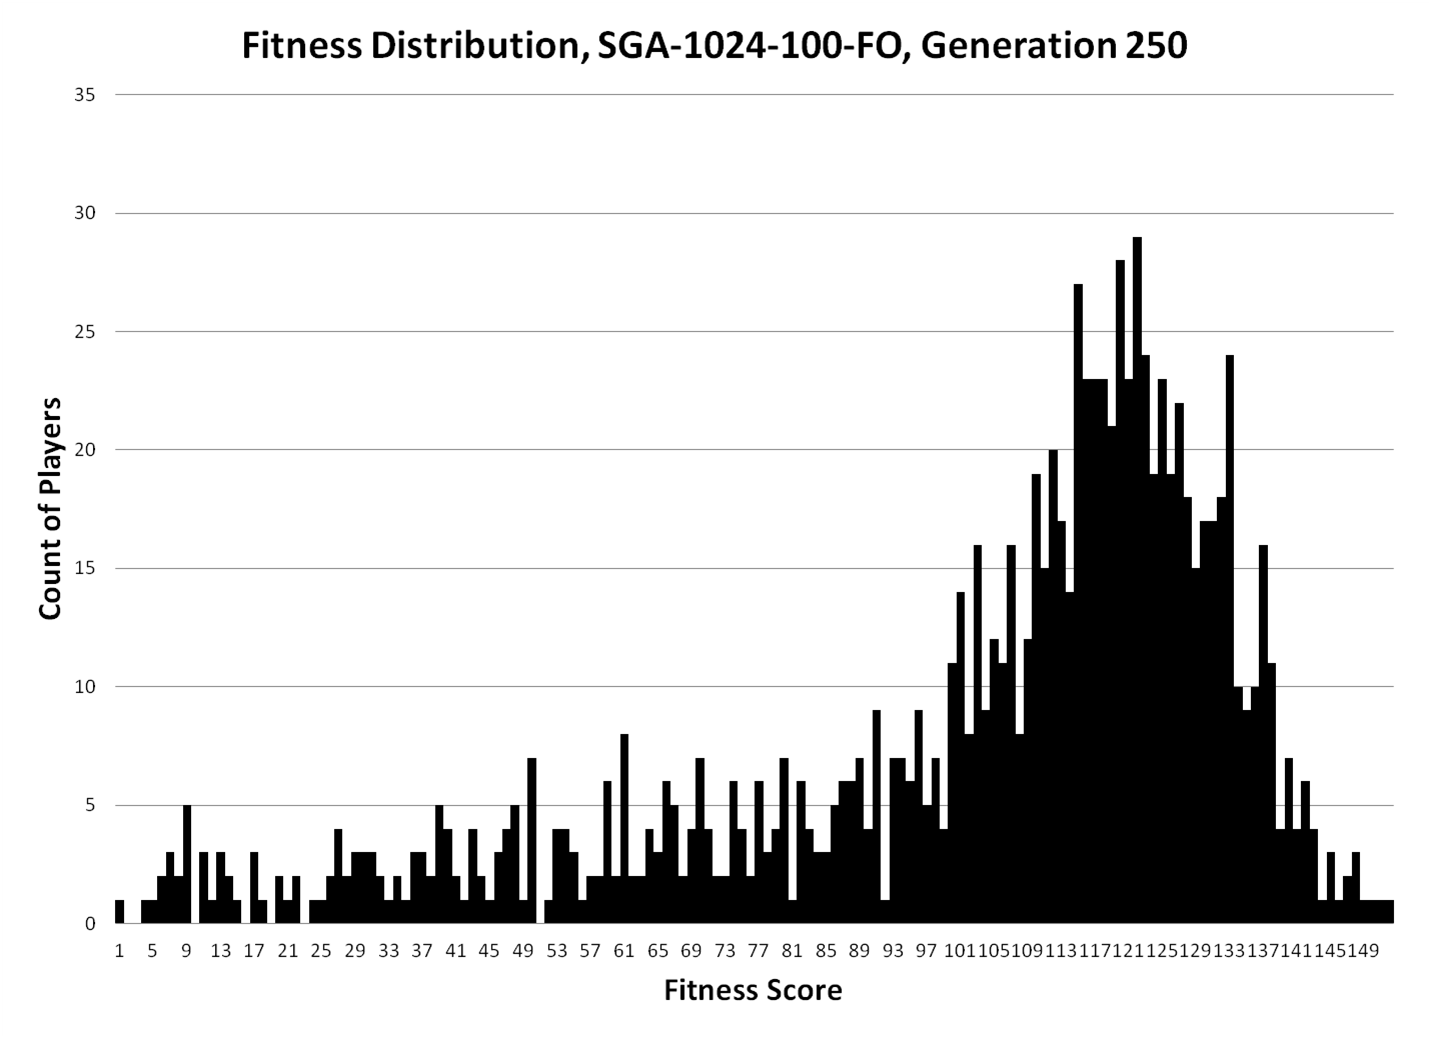
\includegraphics[width=0.75\columnwidth]{Figures/SGA_1024_100_FO_gen250.png}}
\caption[SGA Fitness Generation 289]{This chart shows the fitness
distribution for generation 250 of the SGA-1024-100-FO population.}
\label{figure-sga_gen250}
\end{figure}

Although not shown in this thesis, Generations 500 and 750, for the
SGA-1024-100-FO population, show the same general fitness distribution: a long
tail of low fitness scores, with a peak at higher scores. The fitness
distribution for Generation 999 shows the same pattern and can be seen in
Appendix~\ref{appendix:SGAFitness}.

Appendix~\ref{appendix:SGAFitness} also contains sample fitness distributions
from other SGA populations. They all show the same pattern. At generation 0,
they are generally symmetric, but sometime prior to generation 250, the
distribution skews so that there is a long tail of low fitness scores, and a
peak of scores higher than the expected average.

The descriptive statistics for these populations can be found in
Appendix~\ref{appendix:sgastats}. These tables show in numeric form what is seen
graphically in the figures. The later generations of the SGA populations have a
larger variance in fitness scores, than the earlier generations. Also, the
variance does not appear to monotonically increase, but can be larger or smaller
from one generation sample to another.

The SGA chromosome was designed for these experiments with the assumption that
the SGA chromosomes would perform as well as the RGA or TGA chromosomes. This
was based on previous research in genetic algorithms that proposed that simple
chromosomes would work for most, if not all problems~\cite{goldberg1989genetic}.

Not only did the fitness distributions show problems, but some initial play
testing of a few of the ``best'' SGA players showed that they performed much
more poorly than the RGA and TGA players, losing in every trial. This is likely
due to the increased noise in the chromosome, compared to the RGA and TGA
chromosomes. In the RGA chromosomes, the genes in the chromosome that correspond
to properties that cannot be owned are completely ignored in the game, and have
no effect on other genes during the evolution phase. However, those same genes
in the SGA can and do impact the chromosome in the evolution phase, since
crossover can cause those unused genes to move from an unused part of the
chromosome to a part used for property buying decisions, thus introducing
additional noise into the evolutionary process. These ``junk'' genes appear to
have caused noticeably impaired performance by the SGA chromosomes.

The poor performance of the SGA chromosomes exemplifies Fogel's conclusion
regarding simple chromosomes~\cite{fogel1999intelligence}:

\begin{quote}
We must also admit that several previous theoretical speculations in
evolutionary computation have proven to be incorrect. \ldots~Davis (1991),
Michalewicz (1992), B\"ack and Schwefel (1993), Fogel and Stayton (1994), and
many others, have reported better and faster results in continuous optimization
problems when using real-valued representations instead of bit strings. \ldots
so the proper conclusion is to use the representation that follows naturally
from the problem and gives you the best insight into discovering improved
solutions.
\end{quote}

Based on the poor results of the SGA players, and the conclusion that the
chromosome for a problem should not automatically be a bit string, but should be
one best suited to the problem domain, the effort to improve or validate the SGA
chromosome players was not pursued after the initial evolution phase of this
research.

\subsection{TGA Players} \label{6_TGA}

Finally, the same simulation and evolution was conducted using TGA players. The
results for the TGA player were essentially the same as for the RGA player.

The descriptive statistics for the TGA-*-100-* populations can be found in
Appendix~\ref{appendix:tgastats}. Table~\ref{tab:tga-1024-100-fo-stats} is an
excerpt from the TGA-1024-100-* table in the appendix. As with the RGA
populations, it shows that the variance in fitness is high in early generations,
but it quickly decreases and then remains stable through the last generation.

% Table generated by Excel2LaTeX from sheet 'Stats 1024'
\begin{table}[htbp]
  \centering
  \caption[TGA-1024-100-FO Statistics]{Descriptive Statistics for the TGA-1024-100-FO Population}
    \begin{tabular}{lrrrrrr}
    \toprule
    Population &  Generation & Min    & Max    & Average & Variance & Std Dev \\
    \midrule
    TGA-1024-100-FO & 0      & 99     & 192    & 150.00 & 256.23 & 16.01 \\
    TGA-1024-100-FO & 250    & 118    & 186    & 150.00 & 128.13 & 11.32 \\
    TGA-1024-100-FO & 500    & 113    & 183    & 150.00 & 119.84 & 10.95 \\
    TGA-1024-100-FO & 750    & 110    & 188    & 150.00 & 119.87 & 10.95 \\
    TGA-1024-100-FO & 999    & 108    & 184    & 150.00 & 129.80 & 11.39 \\
    \bottomrule
    \end{tabular}
  \label{tab:tga-1024-100-fo-stats}%
\end{table}%

Of course, not all the populations were as well behaved. Looking at
Table~\ref{tab:app-tga-0032-007-stats} in Appendix~\ref{appendix:tgastats}, it
can be seen that for the TGA-0032-007-* populations the variance does not
decrease over time, but rather appears to fluctuate. The validation experiments
Section~\ref{6_intraPopValidation} will show that this is most likely due to the
small population size (32) and the small number of games (7) played in every
generation.

The fitness distributions for the TGA populations were very similar to the
corresponding fitness distributions for the RGA populations. The player genomes
were also very similar. This is unsurprising, since fitness depends mostly on
buying property (in which the RGA and TGA genomes are identical), and not on
getting out of jail which was the difference between the two genomes.

For this reason, further validation of the TGA players was not pursued after
the initial evolution phase of these experiments. Instead, the remainder of the
study effort focused on validating the RGA players. This validation is discussed
in the next section.

\section{Population Validation} \label{6_Validation}

Validations of the various populations of computer players were performed to
test if the populations were actually getting better. First, populations were
compared across generations. Second, different fitness evaluators were compared.
Finally, the players were validated against human players.

\subsection{Intrapopulation validation}\label{6_intraPopValidation}

For every population, the best player in generation 999 was played against the
best player in generations 250, 500, and 750 for 1000 games. If the population
was actually evolving better players, the best player in the last generation
will win more games on average than the other players; and the best player in
the 250th generation should lose more games on average.

For each game, a fitness score was determined using the finish order fitness
evaluator. The score for each trial was the cumulative fitness over 1000 games.
After 1000 games were played, this same trial was repeated 50 times, without
evolution. The parameters of 50 games repeated for 1000 trials was chosen to
ensure statistically significant results.

\subsubsection{Intrapopulation Validation Results}

Appendix~\ref{appendix:intravalidation} presents the complete set of results for
the RGA-0128 and the RGA-1024 populations. What the tables in the appendix show
is that the populations did improve over time, at least when played against each
other. Table~\ref{tab:validationRGA0128} is an excerpt of the validation results
for the RGA-0128 population (Table~\ref{tab:intrapop128_finorder} in the
appendix).

% Table generated by Excel2LaTeX from sheet 'Finish Order'
\begin{table}[htbp]
  \centering
  \caption{Intrapopulation validation, RGA-0128-100-*, Evaluated by finish
  order}
    \begin{tabularx}{\linewidth}{|p{1in}|p{1in}|r|r|r|r|r|}
    \cline{3-7}
    \multicolumn{1}{l}{} &  & \multicolumn{2}{c|}{Avg fitness} & \multicolumn{3}{c|}{One tailed t test} \\
    \cline{1-7}
    Number of games per generation in original population
    & Original fitness evaluator
    & \multicolumn{1}{p{0.7in}|}{Generation 250}
    & \multicolumn{1}{p{0.7in}|}{Generation 500}
    & \multicolumn{1}{X|}{t test G250 vs G500}
    & \multicolumn{1}{X|}{t test G500 vs G750}
    & \multicolumn{1}{X|}{t test G750 vs G999} \\
    \cline{1-7}
      \multirow{5}{*}{100}
      & FO & 1389.42 & 1489.52 & 0.0000 & 0.0000 & 0.0000 \\
      \cline{2-7}
      & NetW & 1426.96 & 1472.62 & 0.0000 & 0.0000 & 0.0000 \\
      \cline{2-7}
      & NM & 1464.06 & 1494.22 & 0.0001 & \cellcolor{red}0.1532 & 0.0000 \\
      \cline{2-7}
      & NP & 1438.08 & 1487.34 & 0.0000 & 0.0003 & 0.0000 \\
      \cline{2-7}
      & NW & 1418.00 & 1493.70 & 0.0000 & 0.0000 & \cellcolor{red}0.0403 \\
      \cline{1-7}
    \end{tabularx}%
  \label{tab:validationRGA0128}%
\end{table}%

Each row represents a single population. The first row, for example, is a
partial set of the scores and tests for the RGA-0128-100-FO population. The
score in the average fitness column is the average fitness scores for that
player over 50 trials of 1000 games per trial. Since 1000 games are played for
every trial, the expected average fitness score is 1500. The table shows the
average scores for Generation 250 and Generation 500. The average score in
Generation 500 appears to be better than the average score of Generation 250 for
every population, although both players had average fitness less than the
expected average fitness.

To evaluate whether players in later generations were better than players in
earlier generations, a one-tailed Student's t-test was performed with $H_{0}$
that the average fitness is the same for each generation. In most cases, the
null hypothesis is rejected, indicating that the average fitness scores are
different. Since average fitness increases over time, the one-tailed t-test says
that not only are the fitness scores different, the difference in average scores
is statistically significant.

Table~\ref{tab:validationRGA0128} shows 3 of the tests: generation 250 compared
to generation 500, 500 to 750, and 750 to 999. At almost any significance level,
the results indicate that almost every later generation is better than every
earlier generation. The null hypothesis is accepted for only two of the tests in
Table~\ref{tab:validationRGA0128}. One of those is the comparison of generation
500 to generation 750 for the RGA-0128-100-NM population. Accepting the null
hypothesis for that test means that the players from those two generations have
the same ability. The null hypothesis is also accepted when comparing
generaiton 750 to generation 999 for the RGA-0128-100-NW population.

However, looking at all the results in Appendix~\ref{appendix:intravalidation}, 
the null hypothesis is rejected for most of the tests. For the RGA-0128-*-*
populations, the null hypothesis is rejected for 77\% of the tests in
Table~\ref{tab:intrapop128_numwins} and for 76\% of the tests in
Table~\ref{tab:intrapop128_finorder}.

Table~\ref{tab:validationRGA1024} is an excerpt of the validation results
for the RGA-1024 population (Table~\ref{tab:intrapop1024_finorder} in the
appendix).

% Table generated by Excel2LaTeX from sheet 'Finish Order'
\begin{table}[ht]
  \centering
  \caption{Intrapopulation validation, RGA-1024-100-*, Evaluated by finish order}
    \begin{tabularx}{\linewidth}{|p{1in}|p{1in}|r|r|r|r|r|}
    \cline{3-7}
    \multicolumn{1}{l}{} &  & \multicolumn{2}{c|}{Avg fitness} & \multicolumn{3}{c|}{One tailed t test} \\
    \cline{1-7}
    Number of games per generation in original population
    & Original fitness evaluator
    & \multicolumn{1}{p{0.7in}|}{Generation 250}
    & \multicolumn{1}{p{0.7in}|}{Generation 500}
    & \multicolumn{1}{X|}{t test G250 vs G500}
    & \multicolumn{1}{X|}{t test G500 vs G750}
    & \multicolumn{1}{X|}{t test G750 vs G999} \\
    \cline{1-7}
      \multirow{5}{*}{100} 
      & FO & 1434.62 & 1479.22 & 0.0000 & 0.0000 & 0.0000 \\
\cline{2-7}             
      & NetW & 1446.50 & 1476.90 & 0.0000 & 0.0000 & 0.0000 \\
\cline{2-7}     
      & NM & 1453.18 & 1494.18 & 0.0000 & 0.0094 & 0.0000 \\
\cline{2-7}    
      & NP & 1444.48 & 1488.90 & 0.0000 & 0.0042 & 0.0000 \\
\cline{2-7}   
      & NW & 1420.00 & 1477.68 & 0.0000 & 0.0000 & 0.0000 \\
      \cline{1-7}
    \end{tabularx}%
  \label{tab:validationRGA1024}%
\end{table}%

The table shows the average scores for Generation 250 and Generation 500. The
average score in Generation 500 appears to be better than the average score of
Generation 250 for every population, although both players had average fitness
less than the expected average fitness.

Table~\ref{tab:validationRGA1024} shows 3 of the tests: generation 250 compared
to generation 500, 500 to 750, and 750 to 999. The null hypothesis is rejected
for every test in Table~\ref{tab:validationRGA1024}. 

Looking at all the results in Appendix~\ref{appendix:intravalidation}, 
the null hypothesis is rejected for most of the tests. For the RGA-1024-*-*
populations, the null hypothesis is rejected for 80\% of the tests in
Table~\ref{tab:intrapop128_numwins} and for 83\% of the tests in
Table~\ref{tab:intrapop128_finorder}.

\subsubsection{Intrapopulation Validation Summary}

Looking at all the results in Appendix~\ref{appendix:intravalidation}, 
the null hypothesis is rejected for most, but not all, of the tests.

Where the null hypothesis is most often accepted is for populations with a small
number of games per generation, and for populations that are temporally close to
each other. For example, looking at Table~\ref{tab:validationRGA0128-007}
(excerpted from Table~\ref{tab:intrapop128_finorder} in
Appendix~\ref{appendix:intravalidation}), with a significance level of
\(\alpha=0.01\), when the number of games per generation is 7 the null
hypothesis is accepted more than half the time (14 out of 25 trials).

% Table generated by Excel2LaTeX from sheet 'Finish Order'
\begin{table}[htbp]
  \centering
  \caption{Intrapopulation validation, RGA-0128-007-*, Evaluated by finish order}
    \begin{tabularx}{\linewidth}{|p{1in}|p{1in}|r|r|r|r|r|r|}
    \cline{3-8}
    \multicolumn{1}{l}{} &  & \multicolumn{6}{c|}{One tailed t test (\(\alpha=0.01\))} \\
    \cline{1-8}
      Number of games per generation in original population
    & Original fitness evaluator
    & \multicolumn{1}{X|}{t test G250 vs G500} 
    & \multicolumn{1}{X|}{t test G250 vs G750} 
    & \multicolumn{1}{X|}{t test G250 vs G999} 
    & \multicolumn{1}{X|}{t test G500 vs G750} 
    & \multicolumn{1}{X|}{t test G500 vs G999} 
    & \multicolumn{1}{X|}{t test G750 vs G999} \\
    \cline{1-8}
    \multirow{5}{*}{7} 
      & FO & 0.2042 & 0.0140 & 0.4781 & 0.0546 & 0.1618 & 0.0064 \\
\cline{2-8}             
      & NetW & 0.0000 & 0.0108 & 0.1365 & 0.0001 & 0.0000 & 0.0002 \\
\cline{2-8}             
      & NM & 0.0000 & 0.0000 & 0.0000 & 0.4005 & 0.4028 & 0.2877 \\
\cline{2-8}             
      & NP & 0.0000 & 0.0002 & 0.0000 & 0.0289 & 0.4668 & 0.0251 \\
\cline{2-8}             
      & NW & 0.0040 & 0.0001 & 0.0000 & 0.0000 & 0.0000 & 0.0741 \\
    \cline{1-8}
    \end{tabularx}%
  \label{tab:validationRGA0128-007}%
\end{table}%

In addition, an examination of the entire Table~\ref{tab:intrapop128_finorder}
in Appendix~\ref{appendix:intravalidation} shows that the null hypothesis is
accepted most often when comparing Generation 500 to 750 (accepted 9 times out
of 20), and when comparing Generation 750 to 999 (accepted 8 times out of 20).

The conclusion from this set of experiments is that better players evolved in
populations that played large numbers of games per generation. That is, the null
hypothesis is rejected more often for populations that played 100 games per
generation, and less often for populations that played 7 games per generation.

Likewise, in most of the tests, the player from generation 999 was better than
the player from generation 750, which was better than generation 500, which was
better than generation 250. Players in later generations (especially players
that played many games per generation) are better than players in earlier
generations.

\subsection{Interpopulation validation} \label{6_interPopValidation}

Next, the best players from the last generation of similar populations that used
different fitness evaluators were played against each other. This was done to
see which, if any, fitness evaluator produced better players. 

Based on the intrapopulation validation presented previously, this validation
looked at only a single set of populations, the RGA-1024-100-* populations. For
each of the six possible fitness evaluators, the best player from the last
generation of each population was selected for validation. 

The game simulation software can play games with varying numbers of players,
however since the original evolutionary phase was conducted using 4 player
games, it was decided to perform the interpopulation validation with 4 players
for each trial. To do that, the 6 players were permuted into groups of 4 (i.e.,
permutations of 6 items taken 4 at a time, or \(P_{n,k}\)). Each group of 4
players then played 50 games, repeated for 30 trials with no evolution.

For example, one partial permutation might consist of the players that were
evolved using the FO, NP, NM, and TO fitness evaluators. These 4 players
competed in 30 trials of 50 games per trial. Another partial permutation might
consist of the NetW, NM, NP, and NW players which also competed in a separate
set of 30 trials. After each trial, the cumulative fitness score using
Finish Order is recorded. This is performed for all 15 partial permutations of
players.

\subsubsection{Interpopulation Validation Results}

If the fitness evaluators are of equal strength in producing good players, then
the average finish order score for the various players should be the same over
the various trials. What is seen, however, is that this is not the case; some
fitness evaluators do appear to be better than others.

% Table generated by Excel2LaTeX from sheet 'Sheet1'
\begin{table}[htbp]
  \centering
  \caption{Average FO fitness over 50 trials}
    \begin{tabular}{rrrrrrr}
    \toprule
    Round & NW    & FO    & NetW  & TO    & NM    & NP \\
    \midrule
    1     & 79.43 & 80.07 & 72.23 & 68.27 &       &       \\
    2     & 76.70 & 77.07 & 75.03 &       & 71.20 &       \\
    3     & 75.47 & 78.80 & 71.87 &       &       & 73.87 \\
    4     & 79.13 & 78.93 &       & 70.80 & 71.13 &       \\
    5     & 77.13 & 77.33 &       & 69.33 &       & 76.20 \\
    6     & 77.20 & 79.03 &       &       & 70.73 & 73.03 \\
    7     & 83.03 &       & 75.80 & 70.23 & 70.93 &       \\
    8     & 80.07 &       & 76.70 & 69.03 &       & 74.20 \\
    9     & 79.97 &       & 75.27 &       & 72.03 & 72.73 \\
    10    & 79.70 &       &       & 69.13 & 73.27 & 77.90 \\
    11    &       & 84.17 & 76.03 & 69.23 & 70.57 &       \\
    12    &       & 81.20 & 73.63 & 71.73 &       & 73.43 \\
    13    &       & 78.30 & 73.03 &       & 73.10 & 75.57 \\
    14    &       & 79.90 &       & 71.73 & 72.40 & 75.97 \\
    15    &       &       & 79.23 & 69.30 & 72.60 & 78.87 \\
    \bottomrule
    \end{tabular}%
  \label{tab:interpop_avgfitness}%
\end{table}%

50 games are played in each trial, so the expected score for any player is \(50
\cdot 1.5 = 75\). Table~\ref{tab:interpop_avgfitness} shows the actual average
fitness for each player in each round that the player competed.

For example, the first line in Table~\ref{tab:interpop_avgfitness} shows the
average fitness in Round 1 of the validation. The players in that round were the
best player from the last generation of the RGA-1024-100-NW, -FO, -NetW, and -TO
populations (The empty cells for the NM and NP players show that those players
did not compete in Round 1). The table shows each player's average fitness over
the 30 trials using Finish Order.

In the first round, the NW and FO player had average scores greater than
expected, while NetW and TO had average scores lower than expected. Looking at
the column for each player, the NW (number of wins) and FO (finish order)
players had average scores greater than expected in every round. The NetW and NP
player's had greater than expected average scores half the time. The TO and NM
player's always had scores less than expected.

So in general, it can be said that the NW and FO players are probably better
than the NetW and NP players, which are probably better than the TO and NM
players.

Are these differences statistically significant?

As with the intrapopulation validation, a Student's t-test was performed for
each pair of average fitness scores. For each pair, $H_{0}$ is that the pair of
players have the same ability. For each round, 6 t-tests are performed. For the
significance level \(\alpha=0.01\) the null hypothesis is accepted if the
value for that test is greater than 0.01. 

% Table generated by Excel2LaTeX from sheet 'Sheet1 (2)'
\begin{table}[htbp]
  \centering
  \caption{t-test for interpopulation validation for NW}
    \begin{tabular}{rrrrrr}
    \toprule
          & NW v FO & NW v NetW & NW v TO & NW v NM & NW v NP \\
    \midrule
    Round &         &           &         &         &        \\
    1     & 0.3919  & 0.0009    & 0.0000  &         &        \\
    2     & 0.4294  & 0.2068    &         & 0.0106  &        \\
    3     & 0.0427  & 0.0304    &         &         & 0.1922 \\
    4     & 0.4529  &           & 0.0001  & 0.0001  &        \\
    5     & 0.4663  &           & 0.0008  &         & 0.3505 \\
    6     & 0.1769  &           &         & 0.0007  & 0.0211 \\
    7     &         & 0.0007    & 0.0000  & 0.0000  &        \\
    8     &         & 0.0592    & 0.0000  &         & 0.0039 \\
    9     &         & 0.0131    &         & 0.0002  & 0.0011 \\
    10    &         &           & 0.0000  & 0.0023  & 0.2152 \\
    \bottomrule
    \end{tabular}%
  \label{tab:interpop_ttest1}%
\end{table}%

Table~\ref{tab:interpop_ttest1} shows the t-test results for the comparisons of
NW against the other players. For the 6 Rounds in which both NW and FO played
(rounds 1-6), the t-test value is greater than 0.01 in every round, which means
that the null hypothesis is accepted for all comparisons of NW to FO. So the
conclusion is that when the NW or FO fitness evaluators are used to evolve
players, those players have the same fitness.

When comparing NW to TO or NM, the null hypothesis is rejected in all but one
test (Round 2, NW vs NM), and the test that accepts the null hypothesis does so
just barely. The conclusion here is that because the average scores of the NW
player are higher than the average scores of the TO or NM players, the NW
fitness evaluator produces better players than TO or NM.

Finally, for the comparisons between NW and NetW, and NW and NP, the null
hypothesis is accepted for 4 of 6 rounds each. So sometimes, NetW and NP players
can play as well as NW. Note that this generally occurs when one or both of the
TO and NM players are also playing in the round. The ability of NetW and NP to
play as well as NW appears to be due to the presence of weaker players in the
game.

% Table generated by Excel2LaTeX from sheet 'Sheet1 (2)'
\begin{table}[htbp]
  \centering
  \caption{t-test for interpopulation validation for FO}
    \begin{tabular}{rrrrrr}
    \toprule
          & NW v FO & FO v NetW & FO v TO & FO v NM & FO v NP \\
    \midrule
    Trial &        &        &        &        &        \\
    1     & 0.3919 & 0.0019 & 0.0000 &        &        \\
    2     & 0.4294 & 0.1750 &        & 0.0098 &        \\
    3     & 0.0427 & 0.0014 &        &        & 0.0123 \\
    4     & 0.4529 &        & 0.0001 & 0.0001 &        \\
    5     & 0.4663 &        & 0.0003 &        & 0.3079 \\
    6     & 0.1769 &        &        & 0.0000 & 0.0017 \\
    11    &        & 0.0017 & 0.0000 & 0.0000 &        \\
    12    &        & 0.0002 & 0.0000 &        & 0.0004 \\
    13    &        & 0.0030 &        & 0.0009 & 0.0710 \\
    14    &        &        & 0.0001 & 0.0001 & 0.0238 \\
    \bottomrule
    \end{tabular}%
  \label{tab:interpop_ttest2}%
\end{table}%

Table~\ref{tab:interpop_ttest2} shows the t-test results for the FO player
compared to the other players. Column 1, NW vs FO, is the same column seen
earlier in Table~\ref{tab:interpop_ttest1}. The null hypothesis is rejected
(with one exception) for all tests between FO and NetW, TO, and NM. As with NW,
it is accepted in 4 of 6 rounds against NP. So the finish order fitness
evaluator can evolve players of the same ability as number of wins; it is better
at evolving players than net worth, tournament, and number of monopolies; and in
some cases the player created by the number of properties fitness evaluator
performs as well as the finish order player. Again, NP appears to perform as
well as FO because of the presence of weaker players.

The final table, Table~\ref{tab:interpop_ttest3}, shows the remaining t-test
results. The relevant information from that table is that when comparing NetW to
NP, we accept the null hypothesis in every case: The net worth fitness evaluator
results in players equivalent to those created by the number of properties
fitness evaluator. Similarly, TO and NM fitness evaluators result in players of
the same ability. 

The one unusual column is the last column that compares NM to NP where the null
hypothesis is accepted for 5 of 6 rounds. Since a player with many properties is
likely to have many monopolies, it is not surprising that these players and
fitness evaluators would be similar. On the other hand, NP is similar to NetW,
and the null hypothesis was rejected half the time in the tests between NetW and
NM. Most of the tests suggest that, in terms of ability,
\begin{equation*}
NW,FO>NetW,NP>TO,NM
\end{equation*}
So the apparent equivalence between NM and NP appears to be unusual. However,
it appears that the null hypothesis for NM vs NP is usually accepted when there
are other stronger players in the round as well. For example, Round 6 includes 
NW, FO, NM and NP. In this round, it appears that the two strong players, NW and
FO, dominate the results such that the t-test for NM vs NP results in $H_{0}$
being accepted. For Round 15, NetW and NP are the strong players compared to TO
and NM, so $H_{0}$ is rejected for the t-test between NM and NP.

% Table generated by Excel2LaTeX from sheet 'Sheet1 (2)'
\begin{table}[htbp]
  \centering
  \caption{t-test for interpopulation validation for NetW, TO, NM, and NP}
    \begin{tabular}{rrrrrrr}
    \toprule
          & NetW v TO & NetW v NM & NetW v NP & TO v NM & TO v NP & NM v NP \\
    \midrule
    Trial &        &        &        &        &        &  \\
    1     & 0.0390 &        &        &        &        &  \\
    2     &        & 0.0561 &        &        &        &  \\
    3     &        &        & 0.1689 &        &        &  \\
    4     &        &        &        & 0.4371 &        &  \\
    5     &        &        &        &        & 0.0015 &  \\
    6     &        &        &        &        &        & 0.0998 \\
    7     & 0.0010 & 0.0076 &        & 0.3463 &        &  \\
    8     & 0.0004 &        & 0.1403 &        & 0.0079 &  \\
    9     &        & 0.0606 & 0.1289 &        &        & 0.3744 \\
    10    &        &        &        & 0.0372 & 0.0005 & 0.0395 \\
    11    & 0.0025 & 0.0089 &        & 0.2761 &        &  \\
    12    & 0.1392 &        & 0.4582 &        & 0.1894 &  \\
    13    &        & 0.4859 & 0.1214 &        &        & 0.1035 \\
    14    &        &        &        & 0.3505 & 0.0153 & 0.0284 \\
    15    & 0.0000 & 0.0044 & 0.4329 & 0.0754 & 0.0000 & 0.0054 \\
    \bottomrule
    \end{tabular}%
  \label{tab:interpop_ttest3}%
\end{table}%

\subsubsection{Interpopulation Validation Summary}

The results of this set of experiments show that the Number of Wins (NW) and
Finish Order (FO) fitness evaluators produce the best players. It is not
surprising that these two evaluators result in players of similar ability,
since they differ only in the number of points awarded to 2nd, 3rd, and 4th
place in the game. Next, Net Worth (NW) and Number of Properties (NP) produce players
of similar ability, but of less ability than NW and FO. Finally, Tournament (TO)
and Number of Monopolies (NM) produce the least capable players.

These results are also reasonable in terms of the game. Obviously one would
expect high correlation between fitness and the number of games the player can
subsequently win when fitness is measured by NW, FO, or NetW. However there is
less correlation when fitness is measured by NM or NP. Even though a player with
a lot of monopolies or a lot of properties is more able to bankrupt other
players, that ability also depends on which properties or monopolies a player
owns. Suppose there are two players, one with 3 Red properties and the other
with 3 Light Blue properties; they have the same number of properties and the
same number of monopolies, but most experts would say the player with the Red
properties is more likely to win. Similarly, a player with a single high value
monopoly like Red or Orange would be predicted as more likely to win than a
player with two low value monopolies. So there is less correlation between
number of properties or number of monopolies and winning a game.

The apparent weakness of the Tournament fitness evaluator also makes sense in
light of previous research. Panait and Luke found that Single Elimination
Tournament performed worse than K-Random Opponents when noise was introduced
into the solution space~\cite{Panait02acomparative}. The mean number of games
played by each player per match with MSET was only 2 (the median was 5). The low
number of games per generation, and the high degree of randomness in each game,
created a solution space with a large amount of noise, which led to the poor
performance of Tournament fitness evaluator.

Finally, although some of the results imply that NP and NM are similar in
performance, other results imply that NP is better than NM. The fitness
evaluator NP is probably better than NM; the ambiguous results are due to the
confounding effect of having four players per game, rather than a two player
competition. The presence of stronger or weaker players in the set of four
players affects the results of the t-test between any two players.

\section{Human versus Computer Validation}\label{6_humanValidation}

Based on the results of the evolutionary phase of this study, and the intra- and
inter-population validations, a set of RGA players was selected and competed
against human players to validate the evolutionary results. The results of these
competitions are presented here. Although there was a little success by the
computer players, the results are generally disappointing. They do point to
areas where additional research could be conducted.

The intra- and inter-population analysis showed that the best players will be
from the larger populations that played more games per generation, and evolved
under the FO or NW fitness evaluators. For those reasons, players for this
validation were initially selected from the RGA-1024-100-FO population.

\subsection{Human Versus Computer Validation 1}\label{6_humanVRGA1}

For the human versus computer validation, a trading algorithm based on the one
proposed by Yasumura, et al, in ``Negotiation strategy of agents in the MONOPOLY
game'' was implemented~\cite{Yasumura2001Negotiate}.

Full details of the algorithm can be found in Section~\ref{5_trade_property}.
The algorithm evaluates the ownership situation of the properties being traded,
and then sums various combinations of expected gains based on that situation,
and adjusts the sum by a factor \(\omega\). It then adjusts the expected losses
by the factor \(1-\omega\) and subtracts the expected losses from the expected
gains.

When \(\omega\) is close to 1, the player values gains and ignores losses;
alternately, when \(\omega\) is close to 0, the player is more sensitive to
losses. The algorithm results in a value \(U\) which is the adjusted expected
gain (or loss) from the trade.

If the value \(U\) exceeds some threshold, the player proposes the trade, or
accepts the trade. In their paper, Yasumura, et al, claimed that when their
algorithm was compared to the game play of human experts, the algorithm matched
the kinds of trades proposed by human experts when gains and losses were
balanced (\(\omega \approx 0.5\)), and when the threshold was equal to 100. They
also claimed that when competed against each other, their trading agents had the
most wins with low threshold and balanced \(\omega\).

The three best players from the RGA-1024-100-FO population were chosen for the
initial human versus computer validation. For each player, the values for
\(\omega\) and the threshold were set to specific values. Those values are shown
in Table~\ref{tab:val1_params}.

% Table generated by Excel2LaTeX from sheet 'Sheet2'
\begin{table}[htbp]
\centering
\caption{Human vs Computer Validation 1a, Trading Parameters }
\begin{tabular}{lds}	%%zxqdcolumn
 \toprule
 \multicolumn{3}{c}{Trading Parameters} \\
 \midrule
 \multicolumn{1}{l}{Player}  &  \multicolumn{1}{r}{Omega}  
                             &  \multicolumn{1}{r}{Threshold}  \\
 \multicolumn{1}{l}{player0101.dat} &   0.725    &   400   \\
 \multicolumn{1}{l}{player0423.dat} &   0.95     &   300   \\
 \multicolumn{1}{l}{player0667.dat} &   0.65     &   300   \\
\bottomrule
\end{tabular}%
\label{tab:val1_params}%
\end{table}

Each of the three players should have the same relative ability, so different
parameters were used for the trading. Despite the results of Yasumura,
preliminary testing showed that computer players proposed a large number of
trades when the trading parameters were set to a low threshold and balanced
\(\omega\). The values in Table~\ref{tab:val1_params} were chosen to provide a
representative sampling of combinations of trading parameters.

The threshold for all three players is set relatively high, while \(\omega\)
ranges from a somewhat balanced value of 0.65 up to a high of 0.95. These values
were chosen so that the players would favor gains over losses, but would only
propose or accept trades when the gain was significant, thus reducing the number
of proposed trades.

\subsubsection{Human Versus Computer Validation 1 Results}

The human players were instructed to play as many games as possible in a one
week time period. The results are shown in Table~\ref{tab:human_results1a} and
Table~\ref{tab:human_results1b}.

% Table generated by Excel2LaTeX from sheet 'Sheet2'
\begin{table}[htbp]
  \centering
  \caption{Human versus Computer, Trial 1a, Number of Wins}
    \begin{tabular}{lr}
    \toprule
    \multicolumn{2}{c}{Results}\\
    \midrule
    Player  & Number of Wins \\
    \multicolumn{1}{l}{human}          & 53 \\
    \multicolumn{1}{l}{player0101.dat} &  7 \\
    \multicolumn{1}{l}{player0423.dat} &  2 \\
    \multicolumn{1}{l}{player0667.dat} &  8 \\
    \bottomrule
    \end{tabular}%
  \label{tab:human_results1a}%
\end{table}%

% Table generated by Excel2LaTeX from sheet 'Sheet2'
\begin{table}[htbp]
  \centering
  \caption{Human versus Computer, Trial 1a, Average Finish}
    \begin{tabular}{lr}
    \toprule
    \multicolumn{2}{c}{Results} \\
    \midrule
    Player & Average Finish \\
    \multicolumn{1}{l}{human} & 1.5 \\
    \multicolumn{1}{l}{player0101.dat} & 3.0 \\
    \multicolumn{1}{l}{player0423.dat} & 2.8 \\
    \multicolumn{1}{l}{player0667.dat} & 2.7 \\
    \bottomrule
    \end{tabular}%
  \label{tab:human_results1b}%
\end{table}%

It is clear that the human players completely dominated the computer players.
Out of 70 games, the human players won 53 times. The best of the computer
players only managed to win 8 times (\(\approx24\%\)). The average finish order
for the human players was 1.5; the average finish order of the computer players
was \(\approx2.8\)\footnote{Finish order is simply the order of the players at
the end of the game. The winner has a finish order of 1; the second place player
has a finish order of 2, and so on.}. Since the human players won most games,
their average finish order is midway between 1 and 2. The computer players
finished 2nd, 3rd, or 4th most of the time, so their average finish order is
close to 3.

A post validation review was conducted with the human players, and they reported
that some of the reasons for these results were
\begin{enumerate}
  \item {The computer players would often propose trades that gave monopolies to 
  the human player, while getting no monopoly in return.} 
  \item {Similarly, if the human players offered enough cash as part of the 
  trade, the computer players would accept a trade that gave a monopoly to the 
  human but not to the computer player.} 
  \item {The computer players would often propose trades that would give away 
  the second property in a group, rather than trying to get the third property 
  and a monopoly in that group. Subsequently, they would propose a trade that
  reversed the first trade.}
\end{enumerate}
To try to improve the performance of the computer players, the trading algorithm 
was enhanced with some additional rules to try to avoid the situations 
encountered by the human players. In the next validation, the computer players
would avoid trades that gave another player a monopoly unless the computer 
player also got a monopoly from the trade; the computer will also not trade away
a property when the computer owns more than one in the group, unless the trade
would give the computer a monopoly.

In addition, the trading parameters were adjusted as shown in
Table~\ref{tab:val2_params}. The parameters for player 101 were unchanged; for 
the other two players, \(\omega\) was changed so that gains and losses were
evenly weighted. Also, the trading threshold was lowered to 200 for Player 423
and Player 667. The poor performance in the first set of games might be due to
deviating from Yasumura's parameters; modifying the parameters to be closer to
those in Yasumura's paper might result in better performance.

% Table generated by Excel2LaTeX from sheet 'Sheet2'
\begin{table}[htbp]
\centering
\caption{Human vs Computer Validation 1b, Trading Parameters }
\begin{tabular}{lds}	%%zxqdcolumn
 \toprule
 \multicolumn{3}{c}{Trading Parameters} \\
 \midrule
 \multicolumn{1}{l}{Player}  &  \multicolumn{1}{r}{Omega}  
                             &  \multicolumn{1}{r}{Threshold}  \\
 \multicolumn{1}{l}{player0101.dat} &   0.725    &   400   \\
 \multicolumn{1}{l}{player0423.dat} &   0.5      &   200   \\
 \multicolumn{1}{l}{player0667.dat} &   0.5      &   200   \\
\bottomrule
\end{tabular}%
\label{tab:val2_params}%
\end{table}

After these changes were made, The human players competed in another set of
games. The results are shown in Table~\ref{tab:human_results1c} and
Table~\ref{tab:human_results1d}. The human players were again much better than
the computer players, although the computer players may have improved. The
computer players won \(\approx30\%\) of the games this time. Player 667
improved from an 11\% win rate to a 16\% win rate; Player 423 improved from 3\%
to 14\%. Player 101, however, dropped from 10\% to 0\%, hurting the overall
computer rate. Average finish in Table~\ref{tab:human_results1d} shows a similar
improvement: average finish order for the human players became slightly worse,
and improved slightly for the computer players. 

% Table generated by Excel2LaTeX from sheet 'Sheet1'
\begin{table}[htbp]
  \centering
  \caption{Human versus Computer, Trial 1b, Number of Wins}
    \begin{tabular}{lr}
    \toprule
    \multicolumn{2}{c}{Results}\\
    \midrule
    Player  & Number of Wins \\
    \multicolumn{1}{l}{human} & 26 \\
    \multicolumn{1}{l}{player0101.dat} & 0 \\
    \multicolumn{1}{l}{player0423.dat} & 5 \\
    \multicolumn{1}{l}{player0667.dat} & 6 \\
    \bottomrule
    \end{tabular}%
  \label{tab:human_results1c}%
\end{table}%

% Table generated by Excel2LaTeX from sheet 'Sheet1'
\begin{table}[htbp]
  \centering
  \caption{Human versus Computer, Trial 1b, Average Finish}
    \begin{tabular}{lr}
    \toprule
    \multicolumn{2}{c}{Results} \\
    \midrule
    Player & Average Finish \\
    \multicolumn{1}{l}{human} & 1.6 \\
    \multicolumn{1}{l}{player0101.dat} & 2.8 \\
    \multicolumn{1}{l}{player0423.dat} & 2.9 \\
    \multicolumn{1}{l}{player0667.dat} & 2.7 \\
    \bottomrule
    \end{tabular}%
  \label{tab:human_results1d}%
\end{table}%

A post competition discussion was again held with human players. The consensus
feedback from the various human players was that the computer players were
harder to beat in this set of competitions. Some of the players thought the
computer players, while trading better, were still making a few poor trades.

In addition, because of the random feature of the chromosomes, the computer
players were occasionally making poor property decisions compared to a human
player. For example, when a human player lands on a property that would complete
a monopoly, the human will buy the property 100\% of the time. The computer
players, however, will not make the buy decision 100\% of the time, since none
of the gene values evolved to that high of a value. As discussed in
Section~\ref{6_genomeChanges}, some gene values approach 1.0 (which means a
100\% buy decision), but never reach 1.0.

\subsubsection{Human Versus Computer Validation 1 Summary}

This first set of computer versus human validations showed that the computer
players were not up to the level of human players. A large part of
this was due to the trading algorithm that was initially implemented. Another
large factor was due to the phenotype of each player. Even though the
chromosomes tended to result in a high probability of buying decisions (see
Figure~\ref{figure-genome999} for example), that probability is not quite the
same as what a human player would decide. 

So when a human player gets an opportunity to block an opponent's monopoly, they
will take that opportunity 100\% of the time; whereas the computer will block a
monopoly less than that. When a human player gets an opportunity to complete a
monopoly, they will take that opportunity 100\% of the time; the computer will
not.

Also, the poor performance of Player 101 and the better performance of Player
423 and Player 667 seems to suggest that the balanced \(\omega\) and low 
threshold might be better for trading parameters. Player 423 had a high 
\(\omega\) in the first set of competitions and did poorly, wining only two 
games. When \(\omega\) for this player was set to 0.5 and the threshold lowered
to 200, Player 423 won more games. 

On the other hand, while the computer players won 30\% of the games in the
second set of games (better than the 24\% of the first set), they still were not
able to play at the level of human players. 

So even though the balanced parameters used by the players in the second set of
games appeared to improve the computer player's performance they still might not
be the best parameters. It could also be the case that fixing the trading
parameters to specific values might have put those players into a bad position
in the solution space of the game.

Clearly the trading algorithm has a large impact on the performance of the 
computer players, so another attempt was made to improve their performance.

\subsection{Human Versus Computer Validation 2} \label{6_humanVRGA2}

For the second set of tests, the player pool was broadened to include players
from several different generations. The best 4 players from generations 250,
500, 750, and 999 of the RGA-1024-100-FO population were selected. So there were
16 computer players in all. For each game, the program chose 3 opponents at
random. So usually the human player was playing against a mix of players from
the 4 generations.

Another change was that the trading parameters were fixed to exactly follow
Yasumura's recommendations. That is, \(\omega\) was set to be 0.50 and the
threshold was set to be 100 for every player in every game.

Yasumura, et al, claimed that the best agreement with human expert trading was
found with these parameters; they also claimed that when competing against each
other, the computer agents that used those parameters had the most wins
(compared to other computer agents which used different values of \(\omega\)
(0.1, 0.3, 0.7, or 0.9) and different values for threshold (200, 300, 400, or
500).

\subsubsection{Human Versus Computer Validation 2 Results}

A total of 109 games were played between human players and computer players.
Table~\ref{tab:human_rga_2a} shows the number of wins for each computer player,
and the aggregate number of wins for each generation. It also shows how many
games were played by each player and generation, and the percentage wins for
each player and generation.

For example, the first row shows that the players in Generation 250 won 10 out
of 85 games, for a win percentage of 11.8\%. Player 40 won 6 out of 26 games for
a win percentage of 23.1\%.

% Table generated by Excel2LaTeX from sheet 'Pivot table'
\begin{table}[htbp]
  \centering
  \caption{Human versus Computer, Trial 2, Number of Wins}
    \begin{tabular}{rrrr}
    \toprule
    \multicolumn{4}{c}{Results} \\
    \midrule
    Players & Number of wins & Num games & Win \% \\
    \midrule
    \multicolumn{1}{l}{gen250}         & 10.0 & 85 & 11.8 \\
    \multicolumn{1}{l}{player0040.dat} & 6.0  & 26 & 23.1 \\
    \multicolumn{1}{l}{player0191.dat} & 1.0  & 15 & 6.7 \\
    \multicolumn{1}{l}{player0478.dat} & 1.0  & 22 & 4.5 \\
    \multicolumn{1}{l}{player0752.dat} & 2.0  & 22 & 9.1 \\ \\
    \multicolumn{1}{l}{gen500}         & 9.0  & 78  & 11.5  \\
    \multicolumn{1}{l}{player0028.dat} & 2.0  & 25  & 8.0  \\
    \multicolumn{1}{l}{player0445.dat} & 2.0  & 21  & 9.5  \\
    \multicolumn{1}{l}{player0913.dat} & 2.0  & 19  & 10.5  \\
    \multicolumn{1}{l}{player0923.dat} & 3.0  & 13  & 23.1  \\ \\
    \multicolumn{1}{l}{gen750}         & 12.0 & 92  & 13.0  \\
    \multicolumn{1}{l}{player0453.dat} & 1.0  & 28  & 3.6  \\
    \multicolumn{1}{l}{player0474.dat} & 5.0  & 28  & 17.9  \\
    \multicolumn{1}{l}{player0524.dat} & 2.0  & 18  & 11.1  \\
    \multicolumn{1}{l}{player0750.dat} & 4.0  & 18  & 22.2  \\ \\
    \multicolumn{1}{l}{gen999}         & 6.0  & 72  & 8.3  \\
    \multicolumn{1}{l}{player0101.dat} & 1.0  & 18  & 5.6  \\
    \multicolumn{1}{l}{player0423.dat} & 1.0  & 14  & 7.1  \\
    \multicolumn{1}{l}{player0667.dat} & 2.0  & 13  & 15.4  \\
    \multicolumn{1}{l}{player0928.dat} & 2.0  & 27  & 7.4  \\ \\
    \multicolumn{1}{l}{human}          & 72.0 & 109 & 66.1  \\
    \bottomrule
    \end{tabular}%
  \label{tab:human_rga_2a}%
\end{table}%

Compared to the previous set of competitions, on average, the computer players
improved slightly to a win rate of \(\approx34\%\).

What is unexpected though, is that the players in Generation 999 appear to be
worse players than the other generations of computer players. Based on the
intra-population validation (Section~\ref{6_intraPopValidation}), the players
from Generation 999 should have performed better than the other computer
players. Instead, they appear to have performed worse than most other
computer players in this set of competitions.

Table~\ref{tab:human_rga_2b} shows the results for average finish order. As one
would expect based on the number of games won by humans, their average finish
order was between 1 and 2; the average finish order for the computer players was
close to 3.

% Table generated by Excel2LaTeX from sheet 'Pivot table'
\begin{table}[htbp]
  \centering
  \caption{Human versus Computer, Trial 2, Average Finish}
    \begin{tabular}{lr}
    \toprule
    \multicolumn{2}{c}{Results} \\
    \midrule
    Players & Average Finish Order \\
    \multicolumn{1}{l}{gen250} & 2.8 \\
    \multicolumn{1}{l}{player0040.dat} & 2.6 \\
    \multicolumn{1}{l}{player0191.dat} & 2.5 \\
    \multicolumn{1}{l}{player0478.dat} & 3.0 \\
    \multicolumn{1}{l}{player0752.dat} & 3.0 \\
    \multicolumn{1}{l}{gen500} & 2.8 \\
    \multicolumn{1}{l}{player0028.dat} & 2.8 \\
    \multicolumn{1}{l}{player0445.dat} & 2.9 \\
    \multicolumn{1}{l}{player0913.dat} & 2.7 \\
    \multicolumn{1}{l}{player0923.dat} & 2.8 \\
    \multicolumn{1}{l}{gen750} & 2.7 \\
    \multicolumn{1}{l}{player0453.dat} & 2.9 \\
    \multicolumn{1}{l}{player0474.dat} & 2.6 \\
    \multicolumn{1}{l}{player0524.dat} & 2.6 \\
    \multicolumn{1}{l}{player0750.dat} & 2.6 \\
    \multicolumn{1}{l}{gen999} & 2.9 \\
    \multicolumn{1}{l}{player0101.dat} & 3.0 \\
    \multicolumn{1}{l}{player0423.dat} & 3.1 \\
    \multicolumn{1}{l}{player0667.dat} & 2.7 \\
    \multicolumn{1}{l}{player0928.dat} & 3.0 \\
    \multicolumn{1}{l}{human} & 1.6 \\
    \bottomrule
    \end{tabular}%
  \label{tab:human_rga_2b}%
\end{table}%

A post-competition examination of the results leads to the conclusion that the
poor performance of players from Generation 999 in relation to the other players
is probably because the Generation 999 players are more likely to buy
properties. Since they are more likely to buy properties, they are more likely
to have less available cash and also more likely to trade their properties to
the human players. When the human players get a monopoly, it is the Generation
999 players that are more likely to go bankrupt first, since they have less cash
available to pay rents.

A second reason for the poor performance of the Generation 999 players is that,
just by chance, they tended to play more games against players from Generation
750 and less against players from Generation 250. So on average, Generation 999
players tended to play against stronger opponents. In the games in which at
least one other opponent was from Generation 250, the Generation 999 player was
able to finish first or second 50\% of the time.

\subsubsection{Human Versus Computer Validation 2 Summary}

Clearly, for this set of competitions, the human players again greatly
out-played the computer players. The human players won \(\approx66\%\) of the
games they played. 

As with the previous competitions, a major factor is again the property buying
decisions of the computer players: sometimes declining to buy properties to
block an opponent from obtaining a monopoly and sometime declining to buy
properties to complete a monopoly of its own.

It also appears that the trading parameters may have improved the performance of
the computer players. In the first competition, the threshold and \(\omega\)
were fixed at relatively high values, and the computer players won
\(\approx24\%\) of the games. When the threshold was lowered and \(\omega\) made
more balanced, they won \(\approx30\%\) of the games. In this validation, when
the values were set to those recommended by Yasumura, they won \(\approx34\%\)
of the games.

\subsection{Human Versus Computer Validation 3} \label{6_humanVRGA3}

One final validation was performed. For this final validation, the player pool
was again limited to the best players from Generation 999.

Even though Yasumura, et al, claim the best performance from a balanced
\(\omega\) and a low trading threshold, they did not validate these parameters
in a real world situation. The appropriateness of proposals was evaluated by
comparing what the computer proposed for trading to the proposal made by a human
expert in the same situation. In their paper, they indicate that there were some
differences between their computer agents and the human experts, and the reasons
for this difference were that, ``(1) the parameters in the evaluation function
are not tuned enough and (2) the expert is taking into consideration elements
other than the expected profit~\cite{Yasumura2001Negotiate}.'' Similarly,
determining which set of parameters led to the most wins for their computer
players was not tested in real world games, but rather by competing computer
agents against each other. It is also not clear from the paper whether the
computer agents played in 2-player games or multi-player games.

So even though setting \(\omega\) to 0.5 and the threshold to 100 appears to
have improved the performance, these may not be the best parameters. Perhaps
player performance could be improved by allowing the trading parameters to
change from game to game. So the game software was updated to randomly choose
\(\omega\) and the threshold for each player at the start of each game.

The value for the threshold was randomly chosen from the set \{100, 200,
400\} and \(\omega\) was randomly chosen from the set \{0.65, 0.80, 0.95\}. This
value would be different for each player in each game, but would stay constant
for each player during the course of a single game. 

Human volunteers then played the game again. Preliminary results show some
improvement in trading behavior: the computer players propose less trades, and
the trades they do propose are more sensible than they were previously. After a
set period of time, results were gathered from the initial set of games, and the
human players were asked to play a final round of games.

\subsubsection{Human Versus Computer Validation 3 Results}

Looking first at number of wins, Table~\ref{tab:human_results3a} shows that the
number of wins for the human players has increased again to 73\% of the 63 games
played. On the surface, it appears that performance of the computer players has
decreased.

% Table generated by Excel2LaTeX from sheet 'Sheet1'
\begin{table}[htbp]
  \centering
  \caption{Human versus Computer, Trial 3a, Number of Wins}
    \begin{tabular}{lrr}
    \toprule
    \multicolumn{3}{c}{Results}  \\
    \midrule
    Player & Number of Wins & Percent \\
    \multicolumn{1}{l}{player0423.dat} & 2.00   & 3.2\% \\
    \multicolumn{1}{l}{player0928.dat} & 3.00   & 4.8\% \\
    \multicolumn{1}{l}{player0101.dat} & 5.00   & 7.9\% \\
    \multicolumn{1}{l}{player0667.dat} & 7.00   & 11.1\% \\
    \multicolumn{1}{l}{human} & 46.00  & 73.0\% \\
    \bottomrule
    \end{tabular}%
  \label{tab:human_results3a}%
\end{table}%

However, these results are for all the computer players regardless of the values
of the trading parameters. When trading parameters are taken into account, the
picture improves for the computer players.

% Table generated by Excel2LaTeX from sheet 'Sheet1'
\begin{table}[htbp]
  \centering
  \caption{Human versus Computer, Trial 3a, Number of Wins, Omega=0.65, Threshold=400}
    \begin{tabular}{lrr}
    \toprule
    \multicolumn{3}{c}{Results}  \\
    \midrule
    Player & Number of Wins & Percent \\
    \multicolumn{1}{l}{player0928.dat} & 1.00   & 11.1\% \\
    \multicolumn{1}{l}{player0101.dat} & 2.00   & 22.2\% \\
    \multicolumn{1}{l}{player0667.dat} & 2.00   & 22.2\% \\
    \multicolumn{1}{l}{human} & 4.00   & 44.4\% \\
    \bottomrule
    \end{tabular}%
  \label{tab:human_results3b}%
\end{table}%

Table~\ref{tab:human_results3b} shows that when the results are filtered by
\(\omega=0.65\) and threshold=400, the computer players won more than half those
games. Similar improvement is seen in the average finish order values which are
shown in Table~\ref{tab:human_results3c}. The best computer player was Player
101 which had an average finish of 1.67. Player 101 finished 1st or 2nd in every
game it played (with \(\omega=0.65\) and threshold=400), whereas the other
players, including the human players, sometimes finished 3rd or 4th.

% Table generated by Excel2LaTeX from sheet 'Sheet1'
\begin{table}[htbp]
  \centering \caption[Human versus Computer, Trial 3a, Average Finish]{Human
  versus Computer, Trial 3a, Average Finish, Omega=0.65, Threshold=400}
    \begin{tabular}{lr}
    \toprule
    \multicolumn{2}{c}{Results}  \\
    \midrule
    Player & Average Finish Order \\
    \multicolumn{1}{l}{player0101.dat} & 1.67 \\
    \multicolumn{1}{l}{human} & 2.00 \\
    \multicolumn{1}{l}{player0928.dat} & 2.25 \\
    \multicolumn{1}{l}{player0667.dat} & 2.75 \\
    \multicolumn{1}{l}{player0423.dat} & 2.88 \\
    \bottomrule
    \end{tabular}%
  \label{tab:human_results3c}%
\end{table}%

In the final round of games in this validation, the human players continue to
do well, as seen in Table~\ref{tab:human_results3d}, winning almost 59\% of the
41 games that were played. The table shows the results for all games played,
regardless of the trading parameters used by the computer players. The computer
players are slightly better in this round of games (39\% win rate), compared to
the previous round of games (27\% win rate).

% Table generated by Excel2LaTeX from sheet 'Sheet1'
\begin{table}[htbp]
  \centering
  \caption{Human versus Computer, Trial 3b, Number of Wins}
    \begin{tabular}{lrr}
    \toprule
    \multicolumn{3}{c}{Results}  \\
    \midrule
    Player & Number of Wins & Percent \\
    \multicolumn{1}{l}{player0667.dat} & 3.00   & 7.3\% \\
    \multicolumn{1}{l}{player0928.dat} & 4.00   & 9.8\% \\
    \multicolumn{1}{l}{player0101.dat} & 4.00   & 9.8\% \\
    \multicolumn{1}{l}{player0423.dat} & 5.00   & 12.2\% \\
    \multicolumn{1}{l}{human} & 25.00  & 61.0\% \\
    \bottomrule
    \end{tabular}%
  \label{tab:human_results3d}%
\end{table}%

Table~\ref{tab:human_results3e} shows the average finish order results for this
round of games, filtered by \(\omega=0.80\) and threshold=400, and again Player
101 has excelled. Like the previous round in this validation, the average finish
order for Player 101 was 1.67, and it finished every game it played in 1st or
2nd place, much better than the other computer players and the human player.

% Table generated by Excel2LaTeX from sheet 'Sheet1'
\begin{table}[htbp]
  \centering
  \caption{Human versus Computer, Trial 3b, Average Finish Order, Omega=0.80, Threshold=400}
    \begin{tabular}{lr}
    \toprule
    \multicolumn{2}{c}{Results}  \\
    \midrule
    Players & Average Finish Order \\
    \multicolumn{1}{l}{player0101.dat} & 1.67 \\
    \multicolumn{1}{l}{human} & 1.70 \\
    \multicolumn{1}{l}{player0423.dat} & 3.00 \\
    \multicolumn{1}{l}{player0928.dat} & 3.50 \\
    \multicolumn{1}{l}{player0667.dat} & 4.00 \\
    \bottomrule
    \end{tabular}%
  \label{tab:human_results3e}%
\end{table}%

\subsubsection{Human Versus Computer Validation 3 Summary}

In this third validation, the computer players were able to compete at a level
equal to that of the human players. The computer players won 39\% of the games
they played in the final set of validation games
(Table~\ref{tab:human_results3d}); and when filtered for \(\omega\) and
threshold they won a bit more than 55\% of the games in the initial set of this
validation (Table~\ref{tab:human_results3b}). One of the computer players even
played better than the human players in both two sets of games.

The difference between these two sets of games and the previous human versus
computer validations in this chapter is that in this validation the trading
parameters were allowed to fluctuate somewhat randomly. Because of this, the
trading parameters became a partial Genetic Algorithm approach to solving the
problem. The term partial is used because although trading parameters were
chosen at random for each game, they were chosen from a fixed set, and no
evolution of the parameters occurred between games.

These two sets of games also suggest that in real world situations, the trading
parameters that are best are not necessarily those that Yasumura, et al, found
to be best. 

\section{Conclusions}

This chapter has shown that computer players for the game of Monopoly can be
evolved using Genetic Algorithm techniques. The players that evolved did get
better over time, and the Number of Wins and Finish Order fitness evaluators
resulted in the best computer players (at least when competed against each
other). 

Due to the highly random nature of the game, the K-Random opponents technique
for competitive evolutions works best for this solution space, although it does
require a relatively large population and a large number of generations to
evolve better players.

However, although it appears that evolutionary computing can be used to learn
when to make property buying decisions in the game of Monopoly, the computer
players were hampered in this experiment by having a trading algorithm that
sometimes resulted in making bad trades which led to losses against human
players. That is probably partly due to the trading algorithm and partly due to
implementation decisions made when the algorithm was coded. The results here
showed that the conclusions of Yasumura, et al, while valid in the simulated
environment of their implementation, do not work in the real world. 